\documentclass[12pt]{article}
\usepackage{graphicx}
\usepackage{multirow}
\usepackage{authblk}
\usepackage{float}
\usepackage{rotating}
\usepackage{url}
\usepackage{lscape}
\usepackage{longtable}
%\usepackage{subfig}
\usepackage{natbib}
%\usepackage{lineno}
\usepackage{amsmath}
\usepackage{epsfig}
\usepackage{caption}
\usepackage{latexsym}
%\setlength{\captionmargin}{20pt}
%\usepackage{graphicx}
%\usepackage[all,knot]{xy}
%\xyoption{arc}
%\usepackage{url}
%\usepackage{multimedia}
%\usepackage{hyperref}
%\linespread{1.6}
\linespread{1.2}

\newcommand{\Deg}{$^{\circ}$}
\newcommand{\Pic}[2][0.85]{\begin{center}\includegraphics[width=0.8\textwidth,height=#1\textheight,keepaspectratio]{#2}
 \end{center} }
%\newcommand{\captionfonts}{\small}
%%%%%%%%%%%%%%%%%%%%%%%%%%
% Different font in captions
\newcommand{\captionfonts}{\small}

\makeatletter  % Allow the use of @ in command names
\long\def\@makecaption#1#2{%
 \vskip\abovecaptionskip
 \sbox\@tempboxa{{\captionfonts #1: #2}}%
 \ifdim \wd\@tempboxa >\hsize
   {\captionfonts #1: #2\par}
 \else
   \hbox to\hsize{\hfil\box\@tempboxa\hfil}%
 \fi
 \vskip\belowcaptionskip}
\makeatother   % Cancel the effect of \makeatletter
%%%%%%%%%%%%%%%%%%%%%%%%%%%%


\title{Digital Elevation Model (DEM) uncertainty and hazard analysis using a geophysical flow model}
\author[1]{ E. R. Stefanescu }
\author[2]{M. Bursik}
\author[3]{G. Cordoba}
\author[4]{K. Dalbey}
\author[5]{M. D. Jones}
\author[1]{A. K. Patra}
\author[6]{D. C. Pieri}
\author[1]{E. B. Pitman}
\author[2]{M. F. Sheridan}
\affil[1]{Department of Mechanical and Aerospace Engineering, University at Buffalo}
\affil[2]{Department of Geology, University at Buffalo }
\affil[3]{Universidad de Nari\~{n}o, Colombia}
\affil[4]{Sandia National Laboratories, Albuquerque, NM}
\affil[5]{Center for Computational Research, University at Buffalo}
\affil[6]{Jet Propulsion Laboratory, Caltech, Pasadena, CA, 91109 USA}


\date{\today}


\begin{document}
%\linenumbers
\maketitle

\begin{abstract}
  This paper describes a new methodology to quantify the variation in
  the output of a computational fluid dynamics model for block and ash
  flows, when the digital elevation model (DEM) of the terrain and
  other inputs are given as a range of possible values with a
  prescribed uncertainty. Integrating these variations in the possible
  flows as a function of input uncertainties provides well-defined 
  hazard probabilities at specific locations, i.e.,
  a hazard map. Earlier work provided a methodology for assessing
  hazards based on variations in flow initiation and friction
  parameters. This paper extends this approach to include the effect of terrain
  error and uncertainty.
  The results are based on potential flows at Mammoth Mountain,
  California, and Galeras Volcano, Colombia. The analysis establishes 
  the soundness of the approach and the effect of including the uncertainty in DEMs
  on the construction of probabilistic hazard maps.
\end{abstract}

\section{Introduction}

%\subsection{Error modeling and error propagation}

Perhaps the most fundamental product created by field volcanologists
to characterize the potential for destruction of a volcano is the
hazards map.  Often a reasonable hazards map can be made when the
distribution of deposits of a given type are well-exposed, and easily
dated and mapped.  In general, however, difficult logistics or paucity
of previous work may render understanding of a volcano's history quite
incomplete.  Moreover, the depositional record on the flanks of a
volcano cannot often be assumed to be very complete.

Several studies have explored the use of computational fluid
dynamics (CFD) models to produce volcanic hazard maps for a variety of
phenomena at a number of volcanoes \citep{Hooper2003, stinton_2006, murcia_2010, Proctor2010, Sheridan2010}.  Hazard maps for ground-hugging flows that are
constrained by the terrain, such as pyroclastic density currents and
lava flows, are often constructed using a digital representation of the
terrain \citep{Takahashi2000, Keith}.  Usually these terrain
representations are digital elevation models (DEMs).  For this type of
study, terrain elevation is rightly recognized as the most essential
and fundamental of variables in geographic analysis
\citep{Mitasova1996, Atkinson2002, Wechsler2006, stefanescu1}. In earlier work, \citep{Keith}  introduced
procedures for constructing hazard maps using ensembles of CFD model simulations
(the TITAN2D code \citep{Patra2005}) of such flows constructed by
establishing probability distributions of input uncertainties in flow
inititation (location and volumes) and sampling these.  The important
contribution of DEM uncertainty to the variability of the flow
outcomes was not included in that work since there were no readily
available procedures. This work is focused on addressing
this lacuna.


A digital representation of a terrain surface is an approximation of
reality and is often subject to significant error \citep{Mitasova1996}. The error is
usually not known in terms of both magnitude and spatial distribution.
There are in fact large uncertainties associated with the construction
of DEMs. In \citep{Wechsler2006} it was shown that DEMs contain errors
derived from a variety of sources, such as sampling, measurement, and
interpolation, and these errors cannot always be well estimated. When
such DEMs with errors are used in {\it a posteriori} analysis, such as in
simulations of flows, the errors propagate to the predicted flow.

The most important part of DEM error propagation analysis is the
appropriate characterization of the error within the DEM itself,
including information about its distribution and spatial structure
\citep{Shortridge2001}.  DEM vendors generally provide users with a
measure of vertical accuracy in the form of the root mean squared
error (RMSE) statistic. However many papers have reported on the
limitations of a single value of accuracy, stressing that DEM error is
spatially variable and highly correlated \citep{Wechsler2006,
  Amii_Darnell}. Also the magnitude of the DEM error is closely
related to the characteristics of the terrain surface. For example,
slope will influence interpolation procedures.


DEM error propagation analysis was introduced to the GIS 
(Geographic Information System) community in
the early 1990s.  In the work of \citet{Heuvelink1990}, error
propagation in calculating slope and aspect was represented using
Monte Carlo simulation. It was shown
that standard deviations of slope and aspect were higher than
expected.  The effect of error in the DEMs on the erosion models was
emphasized.  A method used by \citet{Qihao_Weng} in quantification of
the uncertainty of DEMs was to create various DEMs using different
interpolation methods and to examine the RMSE from the source map,
sampling and measurement error, and the interpolation process. It was
concluded that RMSE can be used as a general indicator of DEM
uncertainty.  In the literature, DEM error without spatial
autocorrelation was considered to be a worst-case scenario
\citep{Heuvelink1989, VanNiel2004, Oksanen2006}, but no analysis based
on terrain morphology and the effect of different DEMs was done.
\citet{Wechsler2006} developed four different methods for representing
the spatial dependence of error through random fields to assess the
effect on topographic parameters of the DEM uncertainty. The study
showed that uncertainty in the DEM is manifested at higher elevations
in locally steeper slopes, on both slope and elevation maps.
\citet{Florinsky1998} showed that the effect of DEM uncertainty on the
accuracy of slope and aspect estimation cannot be determined by using
data from topographic maps or field surveys, because accurate
derivatives cannot be determined.

One key feature of spatial data is the autocorrelation of observations
in space.  Generally, spatial autocorrelation refers to the
correlation between the same attribute at two locations. Observations
in close spatial proximity tend to be more related than are
observations at larger distance or separation. Errors in spatial data
(such as incorrect elevation values assigned to a point) are spatially
autocorrelated. The effect of correlated DEM error has been
investigated in the literature \citep{Fisher_1991, Goodchild_1992}. It
was shown that not only is error spatially variable throughout a DEM,
but within the elevation model the error value of an individual grid
cell is related to the error in neighboring cells. Unfortunately, DEM
providers do not include information regarding the spatial dependence
or spatial relationship of errors.

Stochastic modeling uses stochastic conditional simulation to generate
multiple equally likely representations of an actual terrain
surface. \citet{Ehlschlaeger_1996, Hunter_Goodchild_1997} computed a
normal distribution of maps or realizations to reproduce the spatial
autocorrelation encountered in the original error surface, filtered
using a Gaussian convolution filter, with kernel sizes derived from
autocorrelation analysis of the original error surfaces.

Various researchers have applied stochastic techniques to evaluate
uncertainty in DEM data. \citet{Ehlschlaeger_1996} stochastically
simulated error in a DEM to evaluate the impact of DEM uncertainty on
a least-cost-path application. \citet{Hunter_Goodchild_1997}
investigated the effect of simulated changes in elevation at different
levels of spatial autocorrelation on slope and aspect
calculations. \citet{Felix_Hebeler} produced uncertainty surfaces to
show the impact of DEM uncertainty on an ice sheet
model. \citet{Amii_Darnell} developed a fuzzy framework to examine the
probable and possible uncertainties in classifying landslide hazard.

The aim of this paper is to quantify the variation in the output of a
computational flow model for block and ash flows, when the model
inputs, including the elevation values represented in the DEM, are
uncertain or given as a range of possible values. Integrating these
variations in the possible flows as a function of input uncertainties
provides well-defined data on the probability of hazard at
specific locations, i.e., a hazard map \citep{Keith}.  In particular,
the focus here is on assessing the influence of DEM uncertainties (along with
uncertainties in initial size and location of the avalanche, and the
internal and bed friction angles).  There is uncertainty in all of
these inputs, which can be represented using either field data or
stochastic methods.  The distribution or the range of the parameters
can be obtained from laboratory and field instruments for friction
angles, and historical records of flow frequency and magnitude for
size of the initial failure.  Stochastic methods are used to assess
the uncertainties in the DEMs: first method consists in a perturbation of the elevation based
on the measured error model, while second method represents an unconditional stochastic
simulation \citep{Ehlschlaeger_1996}.  Both methods generate multiple
likely representations of the actual terrain, while the second one
accounts for the spatial autocorrelation between elevation points.
The effect of DEM uncertainty and its impact on the model output is
analyzed by constructing a hazard map and performing a ``probability
analysis" for two volcanoes with different morphology: Galeras
Volcano, Colombia, and Mammoth Mountain, California, USA.  
The second approach adapted here is based largely on the method of \citet{Ehlschlaeger_1996},
which uses the difference between two independent DEMs to train a
Gaussian model of error.

%\textbf{We review}
In the next sections basic methodology for generating
ensembles of DEMs representative of the true DEM is presented.  Subsequent sections
summarize the TITAN2D flow simulation tool and its use in a systematic
hazard analysis. The hazard analysis tool itself uses ensembles of
TITAN2D simulations to construct statistical surrogate models of flow
outcomes at different locations as a function of model inputs, such as
flow volume, resistance to flow as modeled by a Coulomb frictional
law.  Sampling of these surrogates leads to the construction of
effective hazard maps that reflect the range of uncertainty in the
model inputs.


\section{Methodology}
%\subsection{Stochastic modeling}

In previous work \citep{stefanescu1}, the effect of DEM variability on
the output of TITAN2D %\citep{xxx}
was investigated by comparing an output variable - maximum flow 
depth over the entire time of simulation - from different DEMs of the same site.  These
DEMs were obtained from different techniques at different
resolution. Two types of analysis were performed: a qualitative
analysis and a statistical analysis. The qualitative analysis
consisted of a comparison of the footprint of the flow, extended to a
pixel based classification. The pixels were classified into inundated
and non-inundated classes. For the statistical analysis, a
Kolmogrov -- Smirnov test was performed to assess if two output datasets differed
significantly. The conclusion was that for moderate and smaller scale
flows, use of different DEMs affects computation of accurate
footprints of the flow.

This conclusion motivated the present study, to examine the effect of DEM
uncertainty by creating a model of the error and sampling it to create
an ensemble of possible terrains.  The flow simulation is then run on
every member of this ensemble.

Naive, cell-by-cell approaches to treating DEM uncertainty quickly
lead to the use of thousands if not millions of random variables,
resulting in a computationally infeasible problem.  On the other hand,
the error model described above can be parameterized with one or two
random variables.  The parametrization methods are based on the
assumption that the available DEM is a representation of the terrain
to which errors have been added because of instrumental uncertainty.
Therefore, the DEM can be assumed to be one of an infinite number of
elevation realizations.


\subsection{Method 1} \label{Method1}
In this paper, two ``types'' of DEMs are available of each mountain,
which are used in creating DEM-to-DEM difference maps.  Different
realizations of the terrain were constructed by adding to one DEM --
considered to represent the ``true" elevation -- a ``random''
perturbation.  Since any two types of DEMs are obtained using
different techniques, the difference between them can be added to that
which is assumed to be the ``true" DEM to give a set of possible
DEMs. Thus, the resulting realizations are consistent with the
available set of DEMs. Randomness in the perturbations is created by
multiplying the difference map with a scalar random variable $\xi$, which is normally distributed between 0 and 1.
\begin{equation}
R = M + \xi \cdot Diff
\label{eq:two}
\end{equation}
where $R$ is a realization of the terrain, $M$ is the DEM that best
represents the terrain (the ``true" DEM) and $Diff$ is the difference map. 
In this way we can define a set
of DEM realizations using only one random variable.

\subsection{Method 2}
\label{Method2}

% The second method takes advantage of the various available DEMs of
% different resolutions and different creation methods. The DEM's
% available for experiment are: TOPSAR (5x5m and 30x30m resolution),
% NED (10x10m and 30x30m resolution), SRTM (30x30m and 90x90m
% resolution) and ASTER 30x30m resolution.  By using this method the
% DEM is not an input parameter of the simulator, the effect of DEM is
% accounted by creating a hazard map.  For each DEM we create a hazard
% map, with the same parameter distribution and range as presented
% above.  A final hazard map is created as a weighted sum of the sevene
% hazard map based on how much a particular DEM varied from some
% estimate of the true topography, i.e the "best" DEM
% \citep{stefanescu1}. We divided the DEMs into: 3 categories.  In the
% first category we include the DEMs for which the flow map was very
% different with respect to TOPSAR5m : SRTM90m and interpolated
% TOPSAR30m, in the second category are SRTM30m, ASTER and NED30m,
% while in the last category we include the one which are least
% different: decimated TOPSAR30m and NED10m. This categorization the
% DEMs is used in choosing the appropriate weight for the final hazard
% map.  \textit

For elevation, data at any grid point in a DEM tends to be related to
data from nearby points.  This is the principal motivation of Method
2, based on the work of \citep{Ehlschlaeger_1994}. If more than one
DEM exists for the same location, then difference maps can be
constructed. Such maps are termed error maps
and are generated by subtracting the lower quality DEM from the higher quality DEM (i.e. the ``true'' DEM).
%and characterizes the error of the lower quality DEM at each point. 
These maps are spatially autocorrelated.  Random fields can be used to 
represent these spatially autocorrelated data points.  Let $Z(\mathcal{U})$ be a
continuous random field used to characterize unknown elevation errors
(differences).
% generated by probability distributions which characterize the
% uncertainty of the random variables. $Z$ represents a continuous
% random field and $\mathcal{U}$ represents the area covered by the
% random field.  \textit{Depending on the nature of the terrain, the
%   $Z(\mathcal{U})$ may be continuos, differentiable or many-times
%   differentiable.}
The random field function is implemented in the function
\textit{r.random.surface} \citep{Ehlschlaeger_1994} of GRASS (Geographic Resources Analysis Support System) GIS
\citep{Mitasova1996}, and generates fields obtained using a normal
distribution (mean of 0.0 and variance of 1.0). The random field
function derives its spatial dependence from the use of a distance
based decay filter function. The following equation is used to
generate the random field:
\begin{align}
  &Z(\mathcal{U})= \frac{\sum_v w_{u,v}\epsilon_v}{\sqrt{\sum_v
      w_{u,v}^2}}, \quad u\in \mathcal{U}, \; v \in \mathcal{V}
 \label{eqn1}
 \end{align}
 \begin{align}
   w_{u,v} = \left\{ \begin{array}{ll} 1 & \quad :d_{u,v} \le F \\
       \left(1- \frac{d_{u,v} - F}{D - F} \right)^E & \quad F <
       d_{u,v} \le D, \; u \in \mathcal{U}, \; v \in \mathcal{V}\\ 0 &
       \quad :d_{u,v} > D
\end{array} \right.
\label{eqn2}                                                    
\end{align}
where $\mathcal{V}$ is the set of points potentially influencing
points in a given area, $\mathcal{U}$, $w_{u,v}$ is the spatial
autocorrelative effect between points $u \in \mathcal{U}$ and $v \in
\mathcal{V}$, $\epsilon_v$ is a Gaussian random variable with a mean of 0 and
variance of 1, $d_{u,v}$ is the distance between $u$ and $v$, $D$ is
the minimum distance of spatial independence, $E$ is the distance
decay exponent, and $F$ the distance at which errors are completely
correlated.

A set of random fields is calibrated to the spatial variation of the
field being simulated using a correlogram function. This is done by
fitting the correlogram and choosing the best descriptive parameters
of the random field (the minimum distance of spatial independence, the
correlated distance decay exponent and the filter parameter) in a
weighted least-square estimator implemented in GRASS's
\textit{r.lags.difference}.  After running hundreds of tests with
multiple combinations of $D$, $E$ and $F$, the best random field was 
found by fitting the error map characteristics such that the sum of
least squares difference between an error field's correlogram and the
target correlogram is minimized.
%xx 
Figure~\ref{fig1} shows a sample error map correlogram and several
trial correlograms closely fitting it.  From Eqn ~\ref{eqn2} it can be
seen that the parameters $D$, $E$ and $F$ influence the shape/look of
the correlogram.  It was noted that the main impact of the exponent value
is to characterize the roughness of the texture of the random
surface. Surface roughness decreases as the exponent value gets
closer to 1.0.  Once the parameters are set to a certain value as
determined above one is able to sample from a normal distribution
values for $\epsilon_v$ as given in Eqn ~\ref{eqn1} to generate a
possible perturbation of the provided DEMs. In this way a normal
distribution of possible terrain maps is produced where the mean of
the distribution represents the original DEM used as the ``true''
surface.
% Lag distances less than 1000 meters were weighed twice as important
% than lags greater than 1000 meters, and lag distances less than 100
% meters are weighted five times more importantly xx

The correlogram model was used with sequential Gaussian simulation to
generate a set error map realizations.  Each error realization was added
to the ``true'' DEM indicated as $m(\mathcal{U})$, to generate equally probable realizations of the
topography for the error structure of a DEM under consideration:
\begin{equation}
 R(\mathcal{U})=m(\mathcal{U})+m(m(\mathcal{T}))+(m(s^2(\mathcal{T}))\cdot \epsilon)\cdot Z(\mathcal{U})
\label{eq:one}
\end{equation} 
where $R(\mathcal{U})$ is a realization of the elevation dataset $m(\mathcal{U})$, $\mathcal{T}$ is a
group of sets of spatially uncorrelated sample points in $m(\mathcal{U})$, and $\epsilon$
is a Gaussian random variable with mean 0.0 and variance 1.0. $m(m(\mathcal{T}))$ and
variance $m(s^2(\mathcal{T})$ is mean and variance, respectively, of all sets in 
$\mathcal{T}$. $Z(\mathcal{U})$ specifies the random field as
defined in Eqn ~\ref{eqn1}. Hence, this methodology parameterizes the DEM
using only two Gaussian random variables $\epsilon_v$ and $\epsilon$.

%The error map was
%generated by subtracting the lower quality DEM from the ``true'' DEM,
%and characterizes the error of the lower quality DEM at each point.

\subsection{DEM realizations}

Many DEM users are aware that DEM uncertainty affects the results of
their application, however, in most cases the DEM is accepted as the
true representation of the earth's surface. In this section, two
methods for generating multiple realizations of the terrain are
presented for both Galeras Volcano and Mammoth Mountain, to test
whether it is safe to assume that the representation of topography is
acceptable as it is.

The motivation for creating a process to generate realizations of the DEM was
to incorporate the DEM as one of a host of uncertain input parameters for TITAN2D
simulations and consequent hazard map calculations.  One working hypotheses is that the
DEM contributes a significant proportion of the variance in simulated
flow, hence hazard map output.  For sampling the input parameter
space, a Latin Hypercube Sampling (LHS) was implemented. LHS is
commonly used in compute experiments \citep{McKay1979, Sacks1989} mainly because
it is computationally cheap to generate and can cope with many input
variables. This sampling can have also relative small variance when
measuring output variance. %In the paper of (intern journal) a more detailed
%implementation of LHS is presented. 

For Galeras Volcano, two test DEMs at 30 m spacing were considered for
the analysis. The SRTM (Shuttle Radar Topography Mission) 30m DEM was
derived by spline interpolation from a 90m DEM of southern Colombia
using radar data collected in 2000, while the ASTER (Advanced
Spaceborne Thermal Emission and Reflection Radiometer) DEM was
calculated at the Jet Propulsion Laboratory using orthorectified
imagery from 12 January 2010 (Fig.~\ref{fig2} a).  The ASTER dataset
was used as a surrogate for the ``true'' elevation while the SRTM
dataset was used in creating the error model.


Two 30-m resolution DEMs derived from independent techniques were used
for Mammoth Mountain.  A TOPSAR dataset was considered to be the
``true'' elevation, while an SRTM dataset was used in creating the
error map.  A rectangular area of approximately 42 km$^2$ was
defined within the TOPSAR and SRTM DEMs (Fig.~\ref{fig2} b).

For Method 1, sixty-four (64) DEM realizations were created and used
as input parameters for the TITAN2D simulator along with uncertain
parameters presented in ~\ref{subsec: Model Set-up}.  The input space is defined
by seven parameters. 

% For Method 2 also 64 simulator runs were performed, the input space
% being in this case of 6 parameters.

% The stochastic model developed by \citep{Ehlschlaeger_1996} is
% generating first a error model as the difference between two DEMs
% and then unconditional stochastic simulation is employed to define a
% probability density function (p.d.f.). The p.d.f. generates random
% surfaces with a gaussian distribution matching the mean and standard
% deviation observed in the difference map. The technique does not
% ensure that the "true map" is generated from the process, however it
% does provide a bound within which we can state that true map lies.

As described above for Method 2, realizations of the terrain surface
were created by taking into consideration the spatial autocorrelation
of the error.  The error map was obtained by subtracting the elevation
of a given DEM from the ``true'' elevation at each location. The
correlogram for the difference map was calculated to determine the
range of spatial dependence of elevation points. It was found that spatial
dependence persisted above a threshold value of the correlogram
cross-correlation coefficient of 0.4 to a distance of 2.5 km for
Galeras and 2.1 km for Mammoth. To determine the probability
distribution function (pdf) for the stochastic simulation, 91 sets of
spot locations were selected from the map, each set containing 91
points, all pairs of points were separated by more than 2.5 km or
2.1 km, respectively. For each DEM, pdf statistics were derived.
The random field parameters were chosen after testing more than 400
random field parameters for the smallest difference between the error
model correlogram and the random field.  This occurs when the minimum
distance of spatial independence, $D =2500$; the distance decay, $E =
0.8$, and the filter parameter, $F =400$ for Galeras and $D =2100$, $E
= 0.7$, and $F =350$ for Mammoth.  A total of 64 equally probable
potential elevation surfaces of the area having a 30-m resolution were
generated.

\subsection{Hazard map construction}
%The next step of the analysis is to generate a functional
%representation of the hazard at a location. 
 
There are numerous ways to create a volcanic hazard map based on
computational fluid dynamics modeling.  The traditional Monte Carlo
method can be used if it is assumed that uncertainty in model input
parameters is the main restriction to the knowledge of future events
at a given volcano. This is the case, for example, if it is known that
block and ash flows are common at a given volcano, but it is difficult
to know the size or volume of potential future events.  Although Monte
Carlo is relatively simple to implement, it converges slowly and is
unaffordable computationally because of the number of time-consuming
simulations.  A single TITAN2D run might take 20 minutes on a single
processor. To obtain three-digit accuracy in the expected value of a
specified function would require a million runs. One million runs of
20-min calculations running non-stop on 64 processor would take 217
days \citep{Keith}.

Here, a brief description on the use of an hierarchical emulator that
significantly reduces computational cost is presented; a detailed discussion of the
methodology can be found in \citet{dalbeythesis, Keith}. An emulator
can be thought of as a fast statistical surrogate for a single numerical model
simulation (a simulator). The process of computing a
hazard map for block and ash flows with uncertain model inputs
introduced by \citet{dalbeythesis} is described.  Two-level construction of a group
or ensemble of emulators is used to include a separation of uncertain
inputs and geographic coordinates.  The process starts by identifying
the model inputs whose uncertainties will drive the process. In this
case, the uncertain flow inputs used are volume and shape, starting
location, basal and internal friction angles, and finally topography,
as given by the DEM.  For the resulting eight-dimensional parameter
input space, a Latin Hypercube Sampling was performed to determine
parameter values at which simulations were to be run. As priors for 
the emulator, simulation outputs
for each of these input parameter vectors were stored at 64 grid
points. The sample size is consistent with other numerical experiments
of this type existing in the literature \citep{McKay1979, Sacks1989, Mitasova1996}. 

The output variable of interest for application in this paper is the field of
maximum flow depth over time for each spatial position, at each of the
downsampled input parameter grid points.  Tesselations of the
geographic coordinate space and the parameter input space are
constructed (a Delaunay triangulation was used).  At a designated
location, ${\bf x}^*$, of the input parameter plus spatial coordinate
space at which the hazard is to be computed, the covering simplex
$S_{\bf x}^* $ of the parameter space is identified, and all nodes of
that simplex are enumerated, as are all nodes within a neighborhood
(two hops in the tesselation) of the covering simplex nodes.  For each
such two-hop node, the tesselation was performed in the spatial coordinates followed by an
evaluation of all emulators constructed over these nodes.  These
coordinate space emulators to (the coordinate components of) ${\bf
  x}^*$ by barycentric weighting were averaged; notice there will be an emulator for
each parameter input sample point. Now in the input parameter space,
construct a tessellation of the two-hop nodes and average the
emulators to ${\bf x}^*$ by barycentric weighting of the fine-scale
emulator.  The emulator is now readily and quickly evaluated for each
evaluation. The hazard map construction can now proceed by treating
the emulator as a surrogate for the simulator in the classical Monte
Carlo procedure.  For any point in the domain it can now be exercised the
emulator to get potential flows and hence exceedance probabilities.


\subsection{TITAN2D and flow simulations}

TITAN2D \citep{Patra2005, sheridan_2005} was developed for modeling dry geophysical granular flows,
such as debris avalanches and block and ash flows.  Given a digital
elevation map specifying the topography of a volcano and the values of
input parameters, including the initial volume of erupted material and
the friction angles, TITAN2D calculates the flow depth and velocity at
any location throughout the duration of an event.  The TITAN2D code
combines numerical simulations of a natural granular flow with digital
terrain data. It is based on a depth-averaged model for an
incompressible granular materia governed by Coulomb-type friction
interactions \citep{Savage1989}.  The governing equations are obtained
by applying conservation laws to the incompressible continuum,
providing appropriate constitutive modeling assumptions, and then
taking advantage of the shallowness of the flows (flows are much
longer and wider than they are deep) to obtain simpler depth-averaged
representations \citep{BuPaPi05}. The motion of the material is
considered to be gravitationally driven and resisted by both internal
and bed friction. The stress boundary conditions are: no stress at the
upper free-surface and a Coulomb-like friction law imposed at the
interface between the material and the basal surface.

The primary factor driving the flow is the component of gravity
tangential to the surface, which depends on a local slope computed
from the elevation data, hence, the criticality of the DEM to the flow
computations. The resulting hyperbolic system of equations was solved
using a finite-volume scheme with a second-order Godunov
solver. Although many real geophysical flows --- such as debris flows
--- are fluidized, this study deals only with granular material
that has not been fluidized, such as dome-collapse block and ash flows
or rock avalanches initiated by slope instability.  The program runs
in parallel, using the Message Passing Interface (MPI) to allow
communication between multiple processors, increasing computational
power, decreasing computational time and allowing use of large
datasets. The algorithm uses local adaptive mesh refinement for shock
capturing, and dynamic load balancing for the efficient use of
computational resources. Topographic data are included in the
simulation through a preprocessing routine in which the digital
elevation data are imported.  TITAN2D performs flow simulations on a
DEM of a desired region, the simulation accuracy being highly
dependent on the level of the DEM resolution and quality.

Inputs to the code are the size and location of the initial volume,
the internal and bed friction and the DEM. \citet{Keith} presented
several methods for characterizing the effect of input data
uncertainty on model output. At that time, efficient methods forF
representing the uncertainty associated with spatial parameters like
terrain elevation were not well understood.

\subsection{Bayes Linear Method}

The straightforward way to account for uncertain inputs and stochastic
forcing is a Monte Carlo approach --- run many simulations and
`average' the results in some fashion. If simulations are expensive to
run, this approach is not feasible. To circumvent this difficulty, the
statistics community has developed the idea of an emulator.  In
essence, the emulator is a regression surface based on a
representative sample of simulations at selected inputs, accompanied
by statistical error bounds. Equipped with this surface, output values
at new (untested) input values need not be run.  Instead output
results can be determined by evaluating the emulator. There are indeed
many methods -- kriging, metamodels, support vector machines, by
which such surrogates may be constructed and there exists a body of
literature on the topic \citep{simpson1,simpson2}.  One often-used
emulator is the GAuSsian Process (GASP) emulator, which assumes the
regression has the form of a trend plus a Gaussian
\citep{kennedy2001bcc, ContiOHagan, ohagan2006bac, bayarriusc}. 
\citet{Rougier2008} in his construction of a multivariate emulator 
called the Outer Product Emulator maps 
 the field output directly by including parametric regression terms on the output index.
 To construct a GASP emulator, the covariance structure of the Gaussian
must be assumed and parameters determined by Bayesian or partially
Bayesian methodology.  A fully Bayesian determination of the emulator
can be costly, especially if the input data is high-dimensional.  Here
the Bayes Linear method (BLM) \citep{blm1tutor} to construct an
emulator was used. Given prior beliefs $(B)$ of mean and variance, the BLM
updates these beliefs conditioned on the data $(D)$.  Note that
``data'' generally here refers to the output of computationally
expensive physics based simulators.  Because only the first two
moments of a distribution are determined, the BLM is exact only for
Gaussian distributions.  As an emulator construction, the BLM update
is simpler than a full GASP construction, but the resulting emulator
is comparable.  Given the prior expectation $E[B]$ and variance
$var(B)$, the BLM updates are
\begin{eqnarray} \label{blupdate}
E_D(B) &=& E[B] + cov(B,D) (var(D))^{-1} [D-E[D]] \\ \nonumber
var_D(B) &=& var(B) - cov(B,D) (var(D))^{-1} cov(D,B)
\end{eqnarray}
These update formulae can be derived by minimizing the mean square
error $(B - a^T D)^2$ between $B$ and some linear combination of the
data. Thus the BLM update can be viewed as the projection of the set
of prior beliefs onto the span of the data.

\section{Implementation}
\subsection{Case study I: Galeras Volcano}

Galeras Volcano (elevation 4,276 meters), located in southwestern
Colombia (1\Deg 13.31' N and 77\Deg 21.68' W), is one of the most
active volcanoes on the world \citep{hurtado_1997}. Nearly 400,000
people currently live near the volcano; 10,000 of them reside within
the zone of high volcanic hazard. Pyroclastic flows pose a major
hazard for this population. The current period of activity that began
in 2004 \citep{Smith_Galeras} presents a serious problem for all stakeholders: decision
makers, scientists, public safety officials, and the general
population.  Computational modeling has the potential to provide
useful information for hazard assessment and risk mitigation.
However, there is a need to evaluate the validity of the modeling and
the quality of the DEMs available for use in such modeling.

Galeras is an important volcano for computational flow modeling from
both risk management and scientific perspectives
\citep{calvache1997}. Forecasts of volcanic explosions using various
geophysical tools \citep{narvaez_1997} have occasionally brought
public warnings to a high level of alert during the past 20
years. When the alert reaches the highest level, the public are urged
to evacuate some local areas; this occured as recently as January,
2010 \citep{stefanescu3, Smith_Galeras}. The worst event at Galeras occurred in 1993, when an eruption
killed 9 scientists and journalists \citep{baxter1997}.

The topography of the volcano presents a problem for creation of a
good DEM. The irregular morphology on a small scale, with steep
slopes, narrow channels, deep gorges and abrupt cliffs poses problems
for the creation of accurate topographic models
\citep{ordones_2000}. In addition, the current flow hazard map at
Galeras is mainly based on the sparse geological record
\citep{calvache_1990a}. Dense vegetation, deep erosion, successive
deposits of lava and pyroclastic flows hinder the tracing of specific
deposits in the field. The diverse effects of this landscape, as
reflected in DEMs created by different processes and of different
scales, must be examined and quantified to determine the level of
confidence that can be placed in model results. Galeras provides a
wide range of topographic features that challenge the use of
computational flow models.

\subsection{Case study II : Mammoth Mountain}

Mammoth Mountain is a large, geologically young, composite dome
volcano located on the southwestern rim of Long Valley Caldera,
California \citep{Bailey1989}.  There are many active hazards issues
for Mammoth Mountain, including snow avalanches, rock avalanches and
debris flows. In addition, it is intersected by the Mono-Inyo Craters
volcanic chain, which is the most active volcanic region in the
southwestern U.S.  If Mono-Inyo type activity occurs on Mammoth
Mountain, then domes may form.  These new domes would be growing atop
a steep edifice, and therefore could become gravitationally unstable \citep{Wes2004169, Smith_Mammoth}.
Given that block and ash flows occurred at Mammoth Mountain during its
older dome growth stage, there is reason to believe that renewed dome
formation would result in block and ash flow activity. If this is so,
then parts of Mammoth Lakes, CA, are at risk from block and ash flows.
The previous work on Mammoth Mountain (Stefanescu et al., submitted)
was the testing of the hypothesis that different DEMs result in
different model outputs of block and ash flow inundation.

\subsection{Model Set-up}
\label{subsec: Model Set-up}
In quantifying the DEM uncertainties using TITAN2D, a set
of parameters was drawn on which to set the bounds of the input
domain: internal friction angle, basal friction angle, flow volume,
location and DEM. The numerical values for these parameters were
chosen to bracket the range of flow volumes and initial locations, and
to be representative of the friction angles that have been used by
other researchers in their computational models. 
For the sites used in the study the surface properties and the rheology are 
comparable, which is the main reason why the same reasonable
parameter values were used for both volcanoes.% so they do not
%necessarily represent any optimization for a particular case.  
The internal friction angle has little effect on the output of the flow
models \citep{Keith, sheridan_2005}. Many TITAN2D users have chosen
values of internal friction that range between 15 and 37 degrees with
values between 30 and 35 being the most frequent values used
\citep{Patra2005, murcia_2010}.  For the study, an internal
friction angle uniformly distributed between 20 and 25 degrees was used.

The value of the basal friction angle has a large effect on flow
dynamics in the TITAN2D simulations \citep{Patra2005,
  stinton_2006}. Factors that could affect the choice of basal
friction angle include the volume of the flow, the type of the
pyroclastic flow, the nature of the substrate and the amount of
channelization. \citet{murcia_2010} listed the basal friction values
chosen by TITAN2D users; they range between 5 and 28 degrees; the mean
value being about 15 degrees. It was used a basal friction angle
uniformly distributed between 15 and 20 degrees.
 
Volumes of pyroclastic flows at stratovolcanoes typically cover a few
orders of magnitude. The volume values in this study bracket the range
of possible pyroclastic flows for both Mammoth and Galeras.  According
to \citet{calvache_1990a}, Galeras volcano produced 5 large
pyroclastic flow eruptive episodes; an historic eruption in 1866, and
prehistoric events in 1100, 2300, 2900, and 4500 yBP.  The total
deposit volumes of these episodes range from $\mathcal{O}(10^6 - 9\times 10^6)
m^3$.  Block and ash flows on Mammoth Mountain might contain $\mathcal{O}(10^5 -
10^7) m^3$ of material \citep{Patra2005, Burkett2007}.  Thus, the
choice of volumes ranges from $1.9 \times 10^5$ to $5 \times 10^6
m^3$.  The shape of the initial failure region is approximated as a
paraboloid of radii $r_{max}$, $r_{min}$ and height $h_{max}$. The volume is calculated as $
V=\frac{\pi}{2}\cdot r_{min}\cdot r_{max} \cdot h_{max}. $ For a good
match of the volume range, the radius values were uniformly
distributed between 25 and 500 m, while the initial height followed
the same distribution with values between 10 and 150 m.

Initiation locations were taken from previous mapping of vent sites \citep{Bailey1989},
coupled with knowledge of known weak areas within the volcano as
indicated by hydrothermal alteration.  Around the centers of the
separate initiation locations, different starting positions were
uniformly distributed in a circle of radius 200 m.  A rectangular area
of approximative 40 $km^2$ was defined around the vent within the
available DEMs as the potential run-out area.

\section{Results}

One of the goals of the analysis was to understand the effect of the
spatial structure of available DEMs on hazard maps. Figure~\ref{fig2}
(c) and (d) show the correlograms for the ASTER DEM and the TOPSAR
DEM, which are the DEMs considered to best represent the real
topography for Galeras Volcano and Mammoth Mountain, respectively. It
is apparent that data processing resulted in a smoothing and filtering
of the TOPSAR DEM which causes the correlation coefficient to vary
smoothly as a function of distance and any two elevation values.
Using a distance between two points of 2000m, for the ASTER DEM the
correlation coefficient is 0.6, whereas for the TOPSAR DEM the
correlation coefficient is 0.4. This means that elevation values
within the ASTER DEM are more highly correlated.

Starting from these premises, it can be explained the hazard map output for
the cases when the DEM is considered to be an input parameter for the
TITAND2D model.  Figures~\ref{fig3} (a) and (c)  and Figures~\ref{fig4} 
(a) and (c) display maps of Galeras and Mammoth, respectively, of the 
probability that the flow depth will exceed 0.5 m in the next ten years 
using Method 1 and Method 2 to create the terrain realizations.
 
Figures~\ref{fig3} (b), (d) and ~\ref{fig4} (b), (d) show maps at Galeras and Mammoth of
the spatially varying lack of confidence in the probability hazard map. The lack of
confidence is defined as the computed standard deviation of hazard
probability $\sigma_P$ divided by the hazard probability, $P$.  When
calculated by standard means, as was done here, the ratio $\sigma_P/P$
measures the lack of confidence in the statistic, $P$, due to
insufficient re-sampling of the input parameter space.


Comparison of the figures leads to the conclusion that the
difference between hazard map outputs is more pronounced for Galeras than
for Mammoth Mountain. From the lack of confidence figure it is
observed that in both cases the error is concentrated at the flow margins.

For Mammoth Mountain the differences are less pronounced, but with
important differences again concentrated at the edge of the flow.  An
illustration of how the probabilities vary for Method 1 compared to
Method 2 is shown in Figure~\ref{fig5}. It was observed in comparing every
point where there is a probability of having a flow depth greater than
0.5 m, the results for Galeras show a greater dispersion than do those
for Mountain Mountain.  When the flow is deep, the probability is high
and tends to cluster near unity for both mountains.  As the
probability decreases, dispersion becomes greater for Galeras.  It can be
concluded that as the error map becomes more highly correlated, one
should use a more complex method for creation of topographic
realizations such as stochastic Method 2. It appears that the spatial
autocorrelation of the elevation points influences the hazard map
output and a random perturbation of the elevation such as that used in
Method 1 will not capture this effect.

In a previous work \citep{stefanescu1} it was concluded that for moderate and
smaller-sized flows, different representations of the terrain more
profoundly affect computation of an accurate flow footprint.  For the
present contribution, a new set of hazard maps for the
case wherein the volume is low was built, with a range between $10^4 - 5\times
10^4$ m$^3$ and for the high volume case, using values of $9\times 10^6 - 5\times
10^7$ m$^3$.  Since only 517 spatial cells for Mammoth and 872 cells
for Galeras were included in the flow footprint for the low-volume
case, for any particular cell the probability that the flow would
include that cell tends toward unity (in the case of cells within the
starting region), or zero (in the case of any cell outside of the
starting region but still within the footprint).  Thus the probability
plot is nearly binary, which means that there is a hazard (flow
greater than 0.5m) with either probability $\sim1$ or $\sim0$
Figure~\ref{fig6} (a), (b). It can be observed that there is a significant
mismatch of prediction between the two methods (left upper corner and
right lower corner in both figures) for both volcanoes that can be
critical in the case of a hazards or risk assessment.  For high-volume
flows at Galeras, it was observed that the area of probability greater than
zero is much smaller when Method 2 (topographic error is spatially 
correlated) was used, compared to Method 1 (no correlation of error between
topographic points). This counterintuitive effect needs further study.

The main goal of the study was to explore the effect of DEM uncertainty in
constructing a probabilistic hazards map from a geophysical flow model.  A quantitative and a qualitative analysis
were performed for the case wherein the ``original'' or ``best''
deterministic DEM \citep{stefanescu2} is used as input parameter for the hierarchical
emulator, the output of which is then contrasted with the case wherein
the input is a set of terrain realizations.
Hazard maps produced when DEM uncertainty is not
included were compared to maps produced when DEM uncertainty is included.
Figures~\ref{fig8} and~\ref{fig9} show that for Galeras the
probability that the flow was deeper than 0.5m varies considerably
from the case of no DEM uncertainty. Hence, the DEM is an important
input parameter of which the errors need to be carefully considered in
flow modeling, and the effect of the DEM is not diminished by other
uncertain parameters or the methodology used.  It can be observed that the
uncertainty of having flow greater than 0.5 m increases towards the
flow edge. For Mammoth Mountain, the DEM uncertainty results in more
uncertainty in the flow outline when Method 2 is used. One of the
causes might be that the flow propagates a shorter distance compared
to that in the original DEM.
At Galeras where the autocorrelation is high,  the uncertainty in the 
flow outline increases when correlated DEM error is taken into account. 
In this case, the uncertainty in flow outline increases, suggesting that 
perturbing the DEM is more important as autocorrelation increases.

\section{Conclusions}

Computer models of hazardous phenomena, such as floods, hurricanes and avalanches, are 
 expensive to run, and each run produces an enormous amount data. For example, a flood 
model output may consist of water depth and velocity at every point in a large grid, at every   
time step. Furthermore, these models often require specification of several parameters that may not be 
well characterized, and initial and boundary data that are likewise poorly specified. 
For the first time, in this contribution a process for computing a hazard map due to a geophysical flow with both uncertain model
input parameters and uncertain elevation map, has been described. Uncertainty in the elevation map has been addressed using two methods for creating an ensemble of map realizations with the same error structure as an original elevation model.  In one method, the errors in the model are assumed to be spatially uncorrelated, whereas in the other method, the autocorrelation structure of the error was used to produce the realizations. Once the elevation realizations are produced, the computational model is run over the ensemble of elevation surfaces and outputs are appropriately combined.  The results suggest that it is critical to consider the error autocorrelation structure in the DEM to properly incorporate DEM error in the entire error model and the resulting probabilistic hazards map.

For the two test sites used in this study, one of the main differences is 
the texture of the terrain surface: the digital representation of the surface of Galeras volcano is quantifiably rougher than is the representation of Mammoth Mountain.
An important conclusion for researchers is that, based on the 
surface roughness of the area of study, different methods to asses the uncertainty caused by the DEM
in the flow model can be implemented. In the case of a smooth terrain, for a fast and 
less expensive computational implementation, a simple ``random" perturbation 
method (Method 1) yields results similar to those using the stochastic method (Method 2).
For rough surfaces, the method for creation of separate terrain realizations should include some characterization of the autocorrelation structure in the DEM error.  A 
method based on the error map and an unconditional stochastic simulation as 
presented in this paper is a good option.


\paragraph{Acknowledgments.}  This work was supported by NASA grant
NNX08AF75G.  The work and opinions expressed herein are those of the
authors alone and do not reflect the opinion of NASA.  We are grateful
to JPL for the construction and distribution of the TOPSAR dataset.

\bibliographystyle{plainnat}	
\bibliography{mybib}		

\begin{figure}[H]
\centering
       % \Pic[0.3]{SRTM30_dem.jpg}\\
	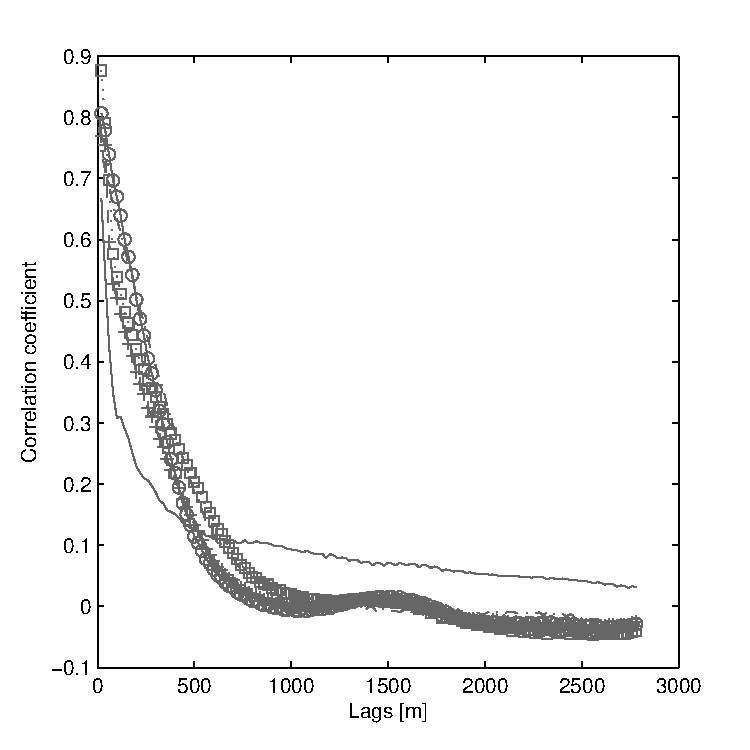
\includegraphics[width=10cm,height=12cm,keepaspectratio]{mammoth_error_correl.pdf}\\       
        \caption{ Error map correlogram (solid line) and various random
          fields fitted to this by choosing different values for the
          parameters $D,E,F$ representing the distances of perfect
          correlation, decay exponent and spatial independence in
          Equation \ref{eqn1}.}
\label{fig1}  
\end{figure}

\begin{figure}[H]
    \begin{minipage}[b]{0.6\textwidth}
        \begin{tabular}{c}
       % \Pic[0.3]{SRTM30_dem.jpg}\\
	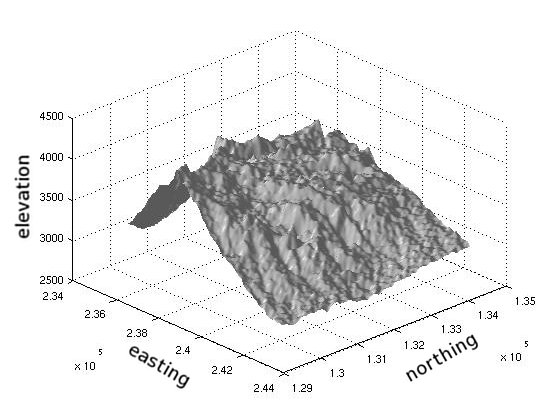
\includegraphics[width=8cm,height=9cm,keepaspectratio]{Aster_galeras.jpg}\\
        (a)
        \end{tabular}
    \end{minipage}
%\hfill
    \begin{minipage}{0.6\textwidth}
        \begin{tabular}{c}
       % \Pic[0.3]{NED30_dem.jpg}\\
	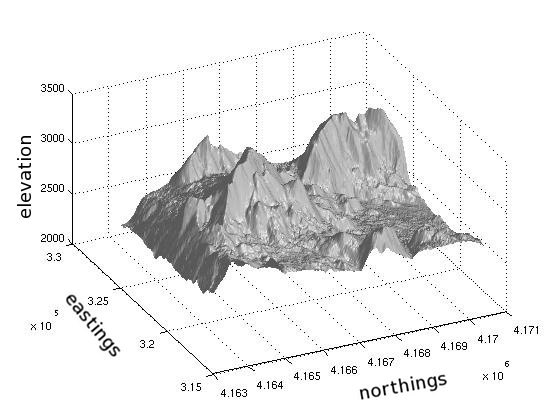
\includegraphics[width=8cm,height=9cm,keepaspectratio]{topsar30m.jpg}\\
        (b)
        \end{tabular}
    \end{minipage} 
    \begin{minipage}[b]{0.6\textwidth}
        \begin{tabular}{c}
       % \Pic[0.3]{SRTM30_dem.jpg}\\
       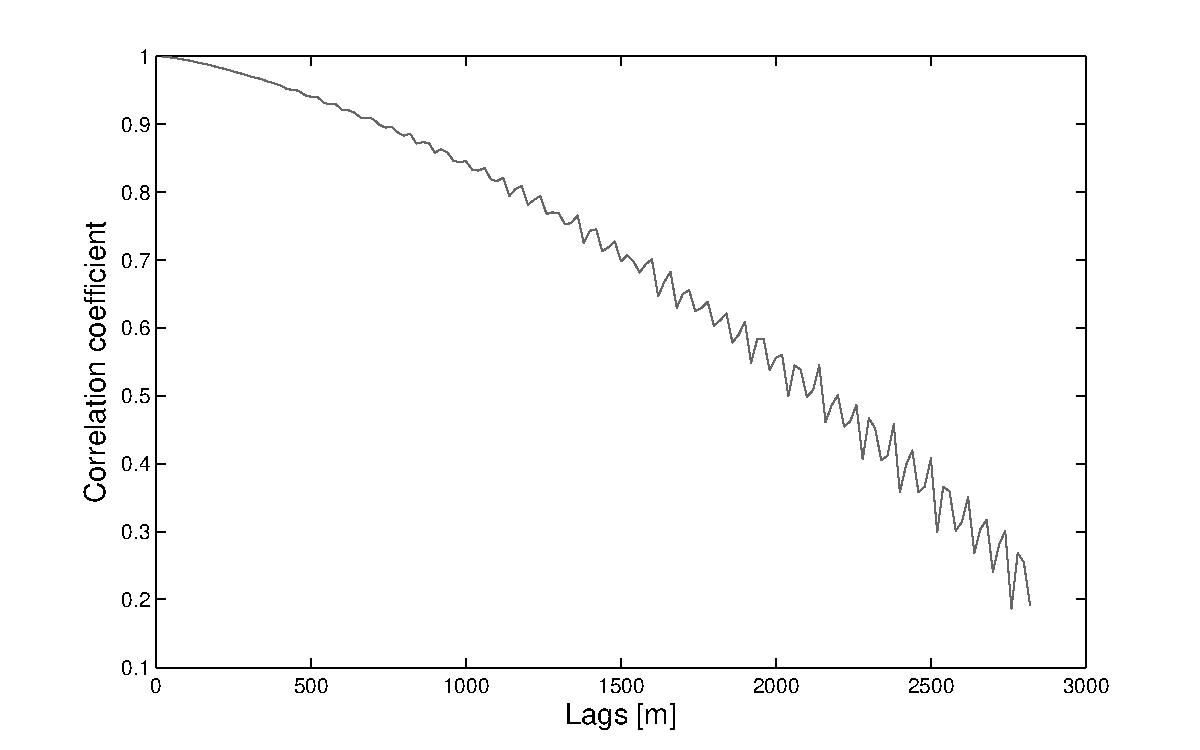
\includegraphics[width=8cm,height=9cm,keepaspectratio]{GalerasAsterCut_correlogram_line.pdf}\\
        (c)
        \end{tabular}
    \end{minipage}
%\hfill
    \begin{minipage}{0.6\textwidth}
        \begin{tabular}{c}
       % \Pic[0.3]{NED30_dem.jpg}\\
	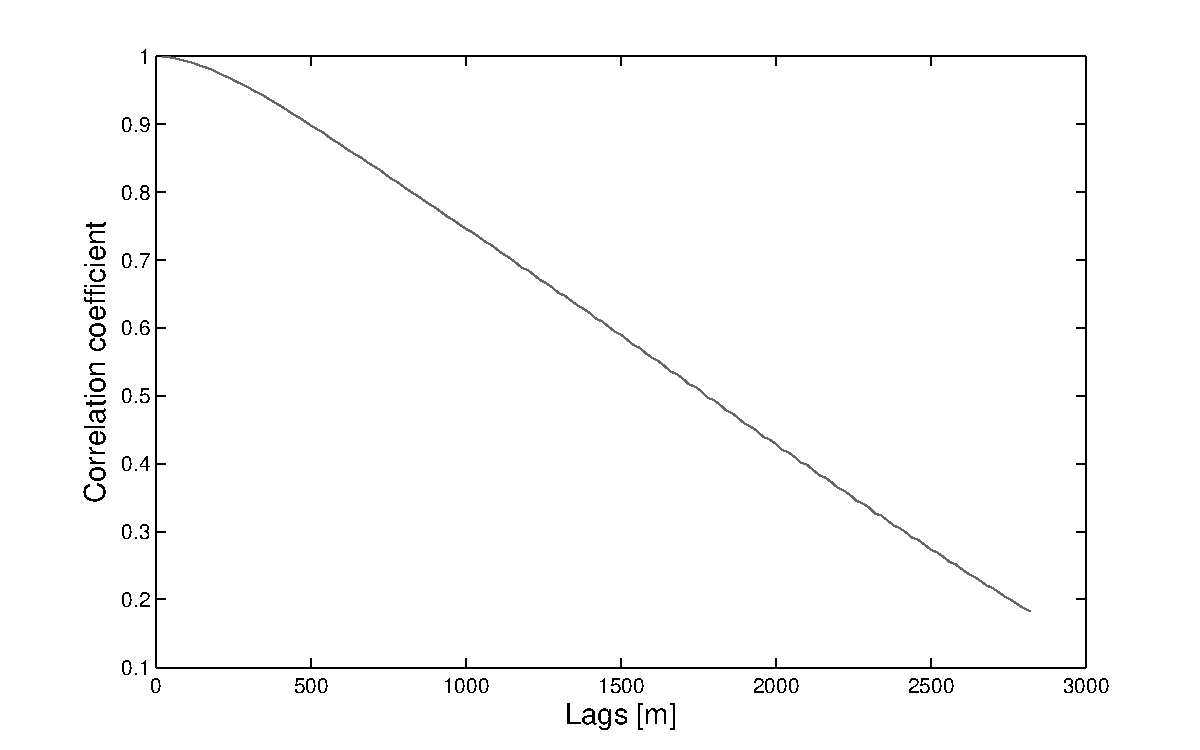
\includegraphics[width=8cm,height=9cm,keepaspectratio]{Mammoth30mCut_correlogram_line.pdf}\\
        (d)
        \end{tabular}
    \end{minipage} 

    \caption{a) The Galeras ASTER 30m DEM terrain surface (Easting,
      Northing and elevation coordinates) (b) The Mammoth TOPSAR 30m DEM
      terrain surface (Easting, Northing and elevation coordinates) (c)
      Galeras Volcano ASTER DEM correlogram (d) Mamouth Mountain
      TOPSAR DEM correlogram}
\label{fig2}  
\end{figure}

\begin{figure}[H]
    \begin{minipage}[b]{0.6\textwidth}
        \begin{tabular}{c}
       % \Pic[0.3]{SRTM30_dem.jpg}\\
       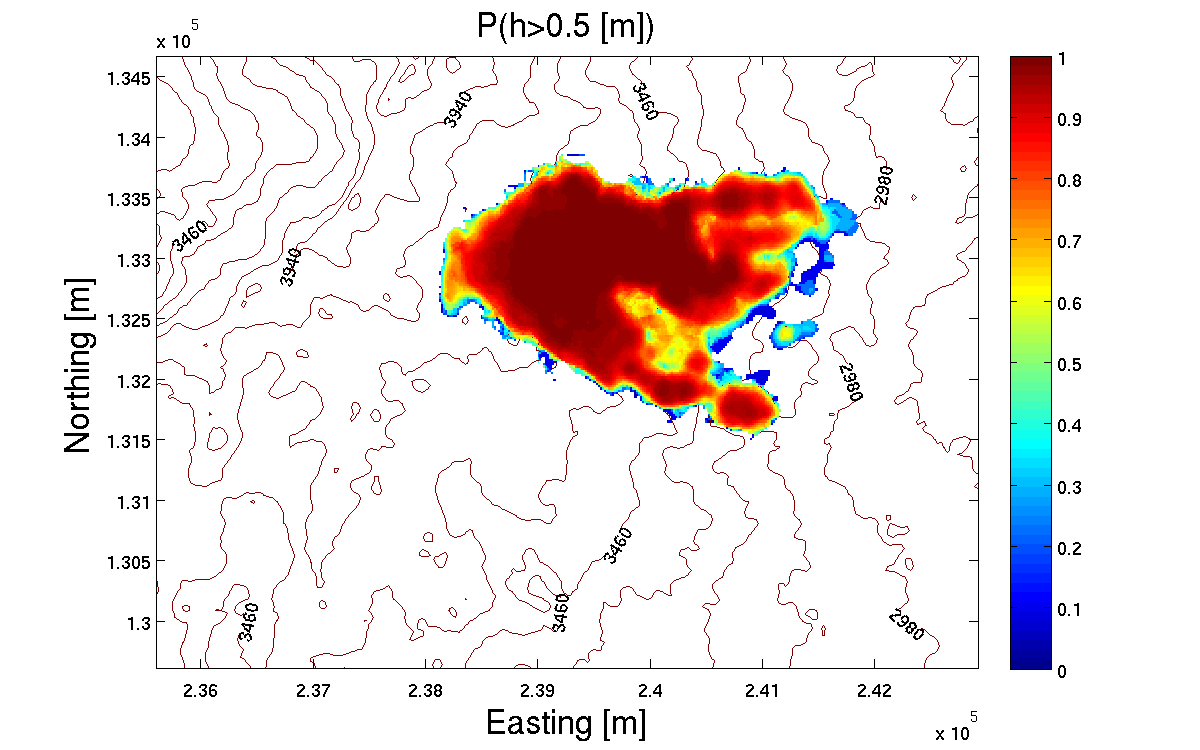
\includegraphics[width=8cm,height=9cm,keepaspectratio]{Galeras_0_P.pdf}\\
        (a)
        \end{tabular}
    \end{minipage}
%\hfill
    \begin{minipage}{0.6\textwidth}
        \begin{tabular}{c}
       % \Pic[0.3]{NED30_dem.jpg}\\
	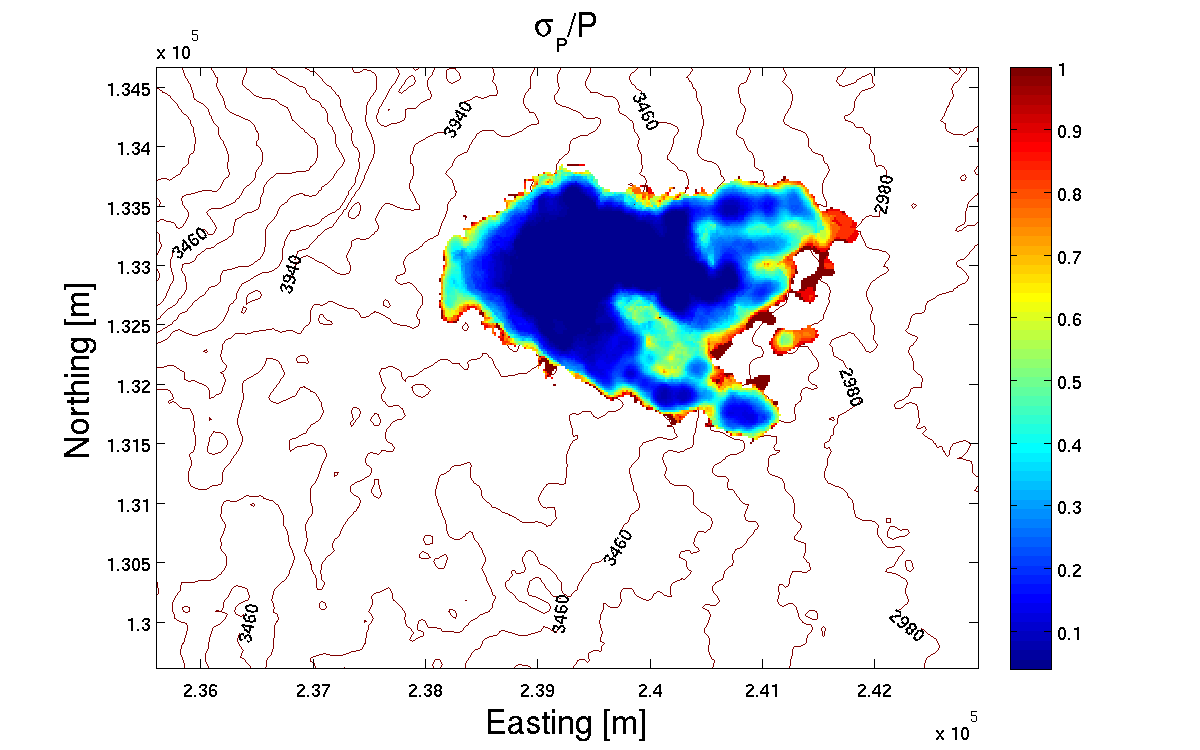
\includegraphics[width=8cm,height=9cm,keepaspectratio]{Galeras_0_sigma.pdf}\\
        (b)
        \end{tabular}
    \end{minipage} 
        \begin{minipage}[b]{0.6\textwidth}
        \begin{tabular}{c}
       % \Pic[0.3]{SRTM30_dem.jpg}\\
       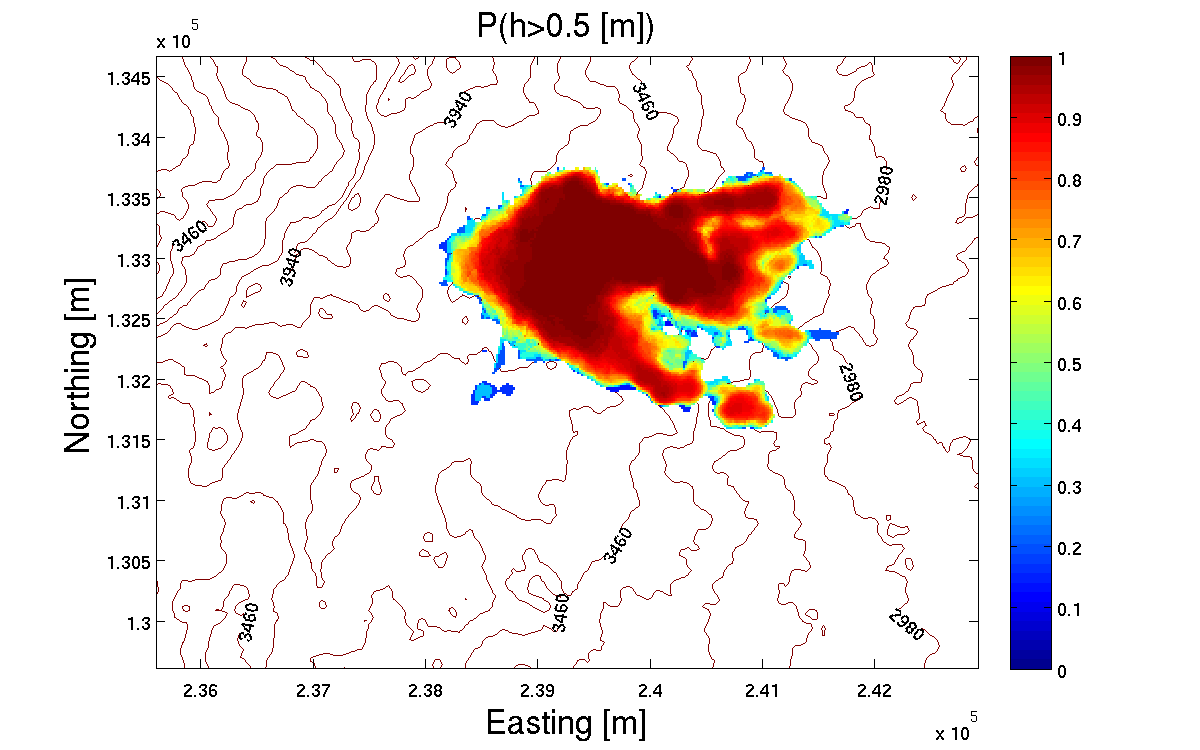
\includegraphics[width=8cm,height=9cm,keepaspectratio]{Galeras_3_P.pdf}\\
        (c)
        \end{tabular}
    \end{minipage}
%\hfill
    \begin{minipage}{0.6\textwidth}
        \begin{tabular}{c}
       % \Pic[0.3]{NED30_dem.jpg}\\
	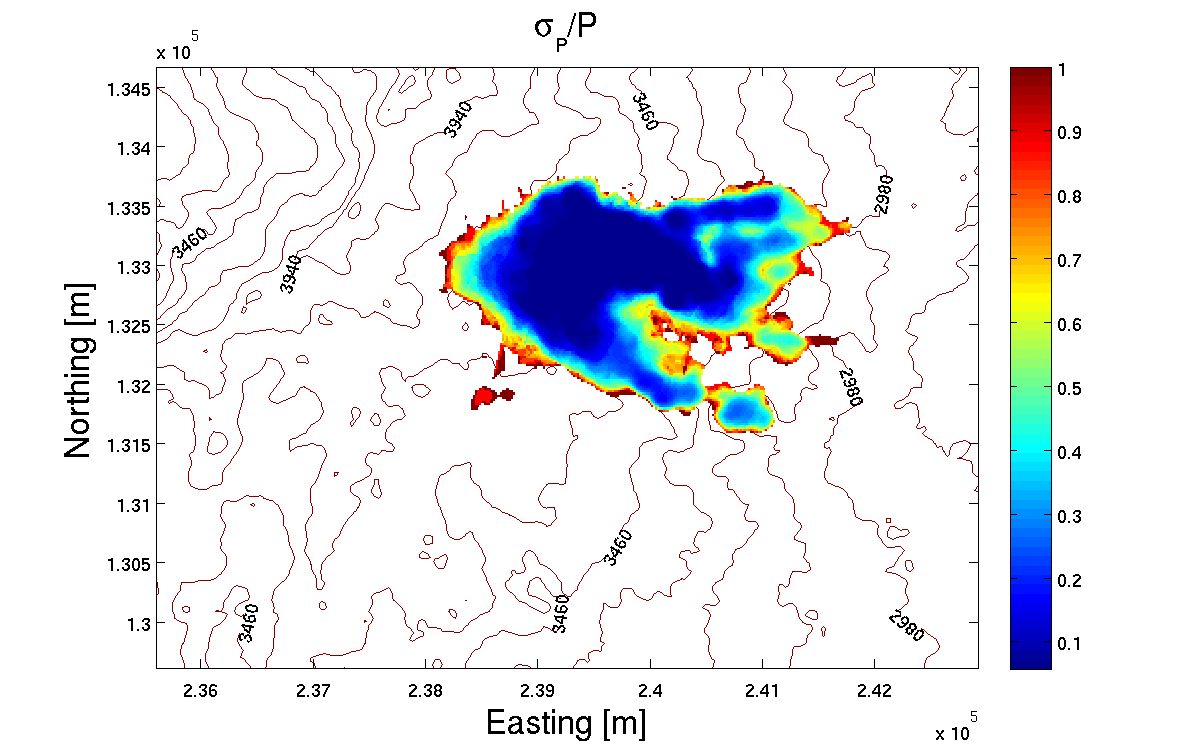
\includegraphics[width=8cm,height=9cm,keepaspectratio]{Galeras_3_sigma.pdf}\\
        (d)
        \end{tabular}
    \end{minipage} 
    \caption{a) Probability that a flow will exceed 0.5 m in depth as
      a function of position on Galeras Volcano, Columbia, given the
      uncertainties in DEM and input parameters using Method 1 to
      create DEM realizations (b) Standard deviation in the estimate
      that the flow will exceed 0.5 m in depth -- Method 1 (c)
      Probability that a flow will exceed 0.5 m in depth as a function
      of position on Galeras Volcano, Columbia, given the
      uncertainties in DEM and input parameters using Method 2 to
      create DEM realizations (d) Standard deviation in the estimate
      that the flow will exceed 0.5 m in depth -- Method 2}
\label{fig3}  
\end{figure}

\begin{figure}[H]
    \begin{minipage}[b]{0.6\textwidth}
        \begin{tabular}{c}
       % \Pic[0.3]{SRTM30_dem.jpg}\\
       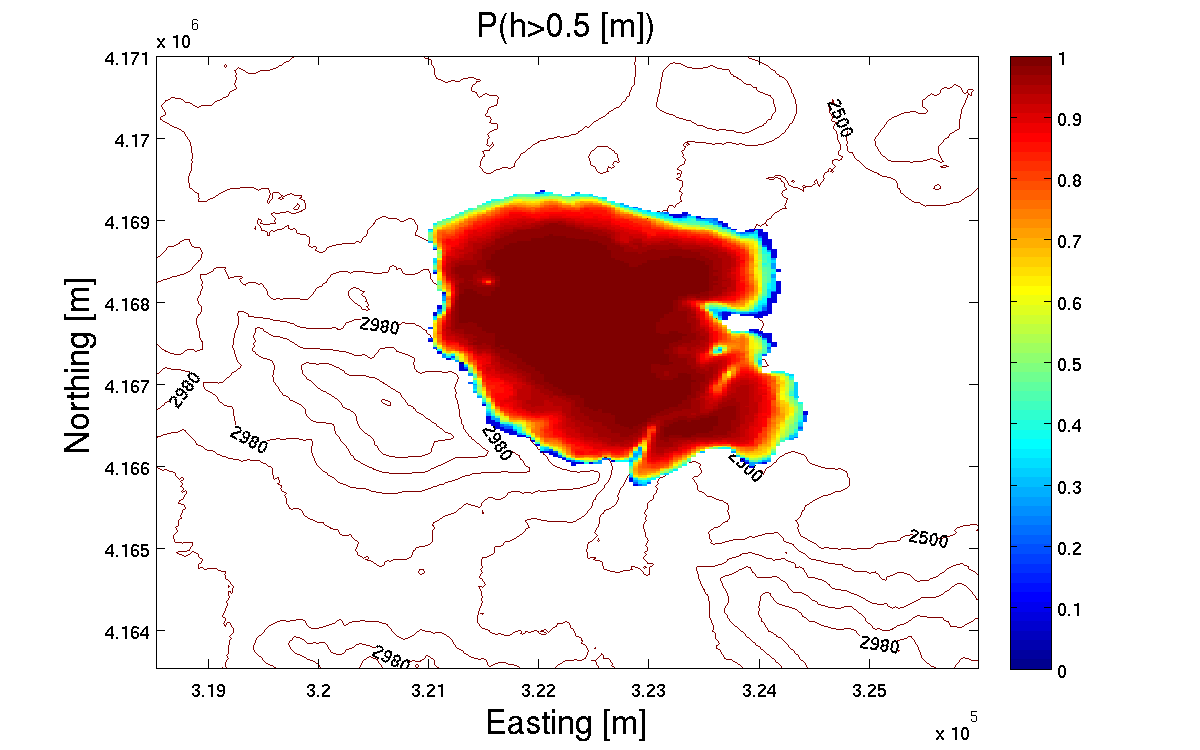
\includegraphics[width=8cm,height=9cm,keepaspectratio]{Mammoth_0_P.pdf}\\
        (a)
        \end{tabular}
    \end{minipage}
%\hfill
    \begin{minipage}{0.6\textwidth}
        \begin{tabular}{c}
       % \Pic[0.3]{NED30_dem.jpg}\\
	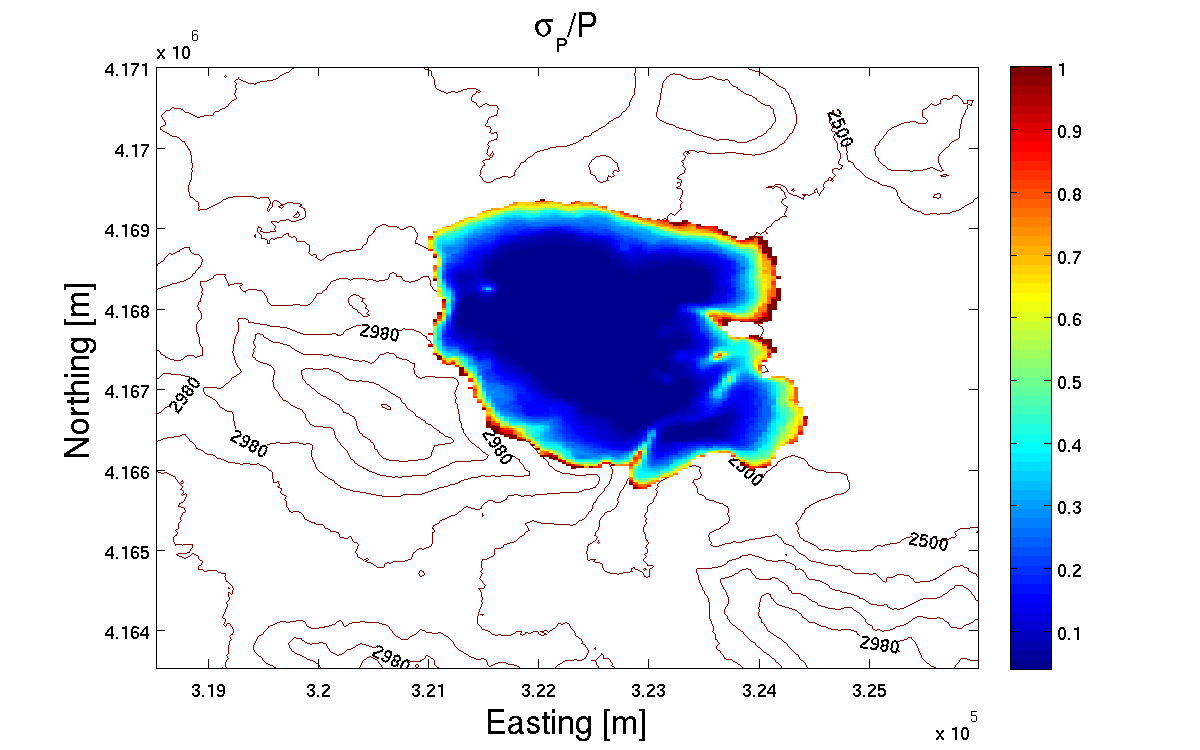
\includegraphics[width=8cm,height=9cm,keepaspectratio]{Mammoth_0_sigma.pdf}\\
        (b)
        \end{tabular}
    \end{minipage} 
        \begin{minipage}[b]{0.6\textwidth}
        \begin{tabular}{c}
       % \Pic[0.3]{SRTM30_dem.jpg}\\
       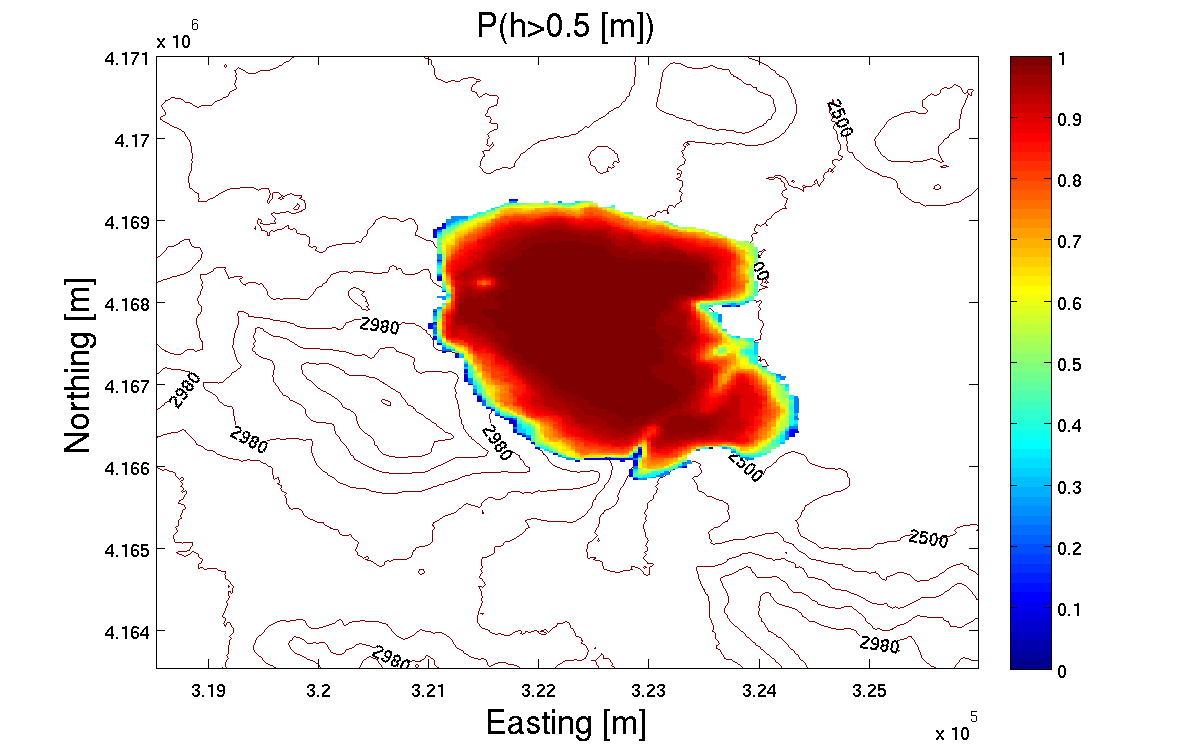
\includegraphics[width=8cm,height=9cm,keepaspectratio]{Mammoth_3_P.pdf}\\
        (c)
        \end{tabular}
    \end{minipage}
%\hfill
    \begin{minipage}{0.6\textwidth}
        \begin{tabular}{c}
       % \Pic[0.3]{NED30_dem.jpg}\\
	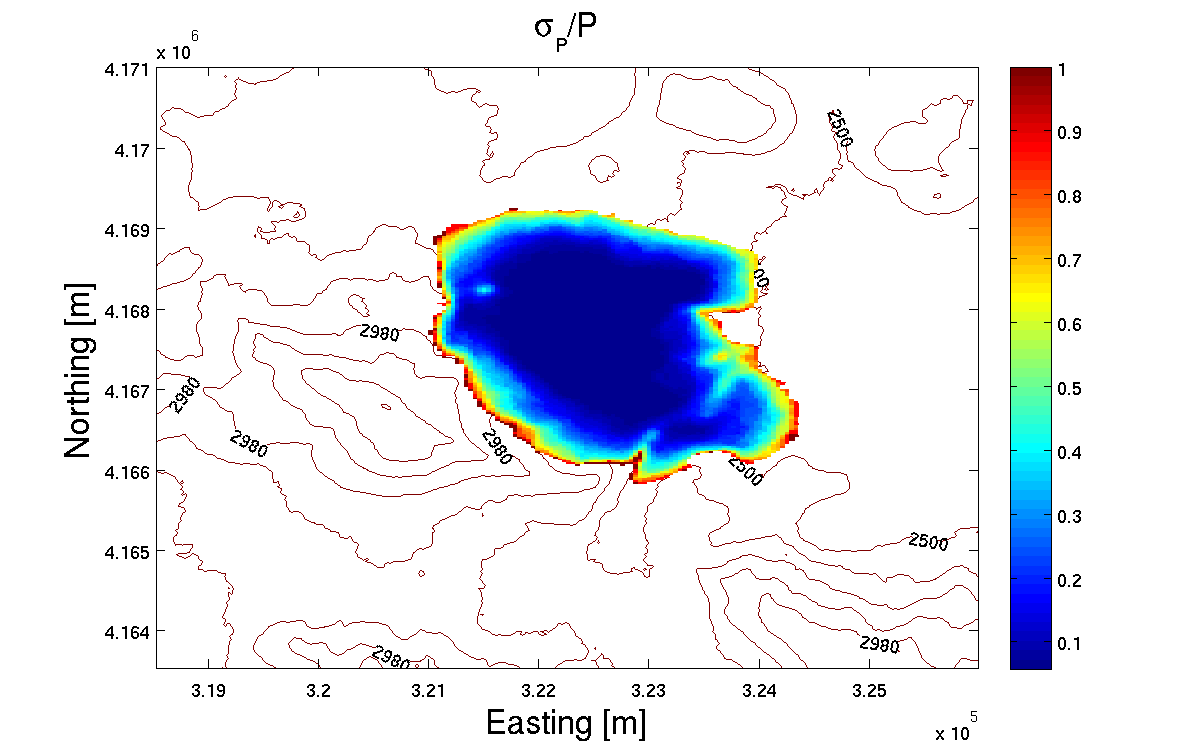
\includegraphics[width=8cm,height=9cm,keepaspectratio]{Mammoth_3_sigma.pdf}\\
        (d)
        \end{tabular}
    \end{minipage} 
    \caption{a) Probability that a flow will exceed 0.5 m in depth as
      a function of position on Mammoth Mountain, CA, given the
      uncertainties in DEM and input parameters using Method 1to
      create DEM realizations. (b) Standard deviation in the estimate
      that the flow will exceed 0.5 m in depth -- Method 1 (c)
      Probability that a flow will exceed 0.5 m in depth as a function
      of position on Mammoth Mountain, CA, given the uncertainties in
      DEM and input parameters using Method 2 to create DEM
      realizations.  (b) Standard deviation in the estimate that the
      flow will exceed 0.5 m in depth -- Method 2 }
\label{fig4}  
\end{figure}


%see /rainier1/data/ers32/Research_Ramona/second_paper_code/temp_plot/low_and_high 

\begin{figure}[H]
    \begin{minipage}[b]{0.6\textwidth}
        \begin{tabular}{c}
       % \Pic[0.3]{SRTM30_dem.jpg}\\
       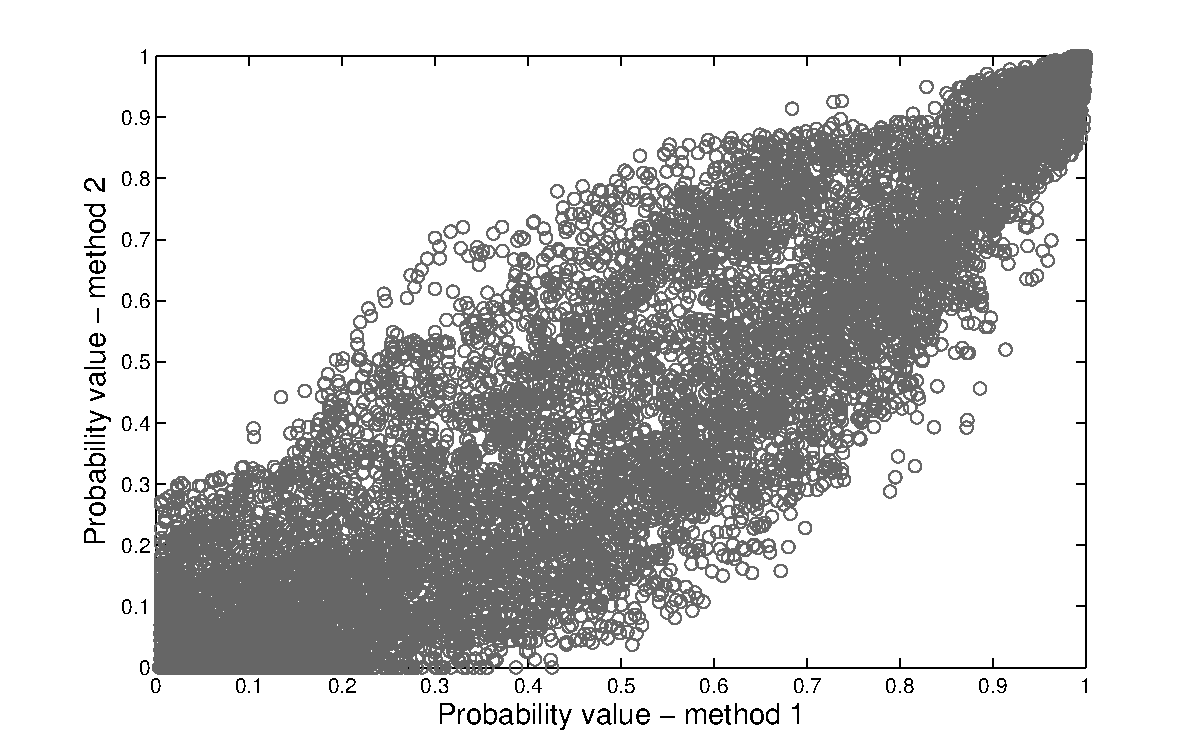
\includegraphics[width=8cm,height=9cm,keepaspectratio]{cloud_galeras.pdf}\\
        (a)
        \end{tabular}
    \end{minipage}
%\hfill
    \begin{minipage}{0.6\textwidth}
        \begin{tabular}{c}
       % \Pic[0.3]{NED30_dem.jpg}\\
	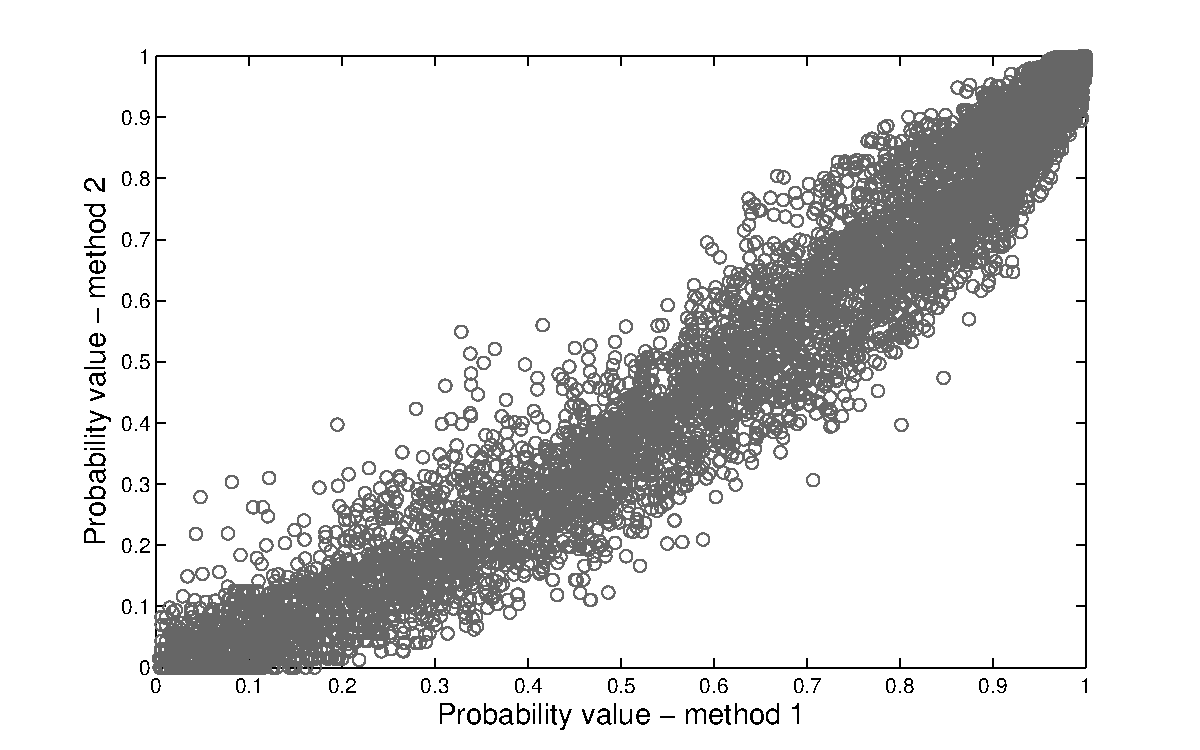
\includegraphics[width=8cm,height=9cm,keepaspectratio]{cloud_mammoth.pdf}\\
        (b)
        \end{tabular}
    \end{minipage} 
    \caption{a) The probability that flow will exceed 0.5 m Method 1
      versus Method 2 for Galeras Volcano, Colombia (b) The
      probability that flow will exceed 0.5 m Method 1 versus Method 2
      for Mammoth Mountain, CA }
\label{fig5}  
\end{figure}

\begin{figure}[H]
    \begin{minipage}[b]{0.6\textwidth}
        \begin{tabular}{c}
       % \Pic[0.3]{SRTM30_dem.jpg}\\
       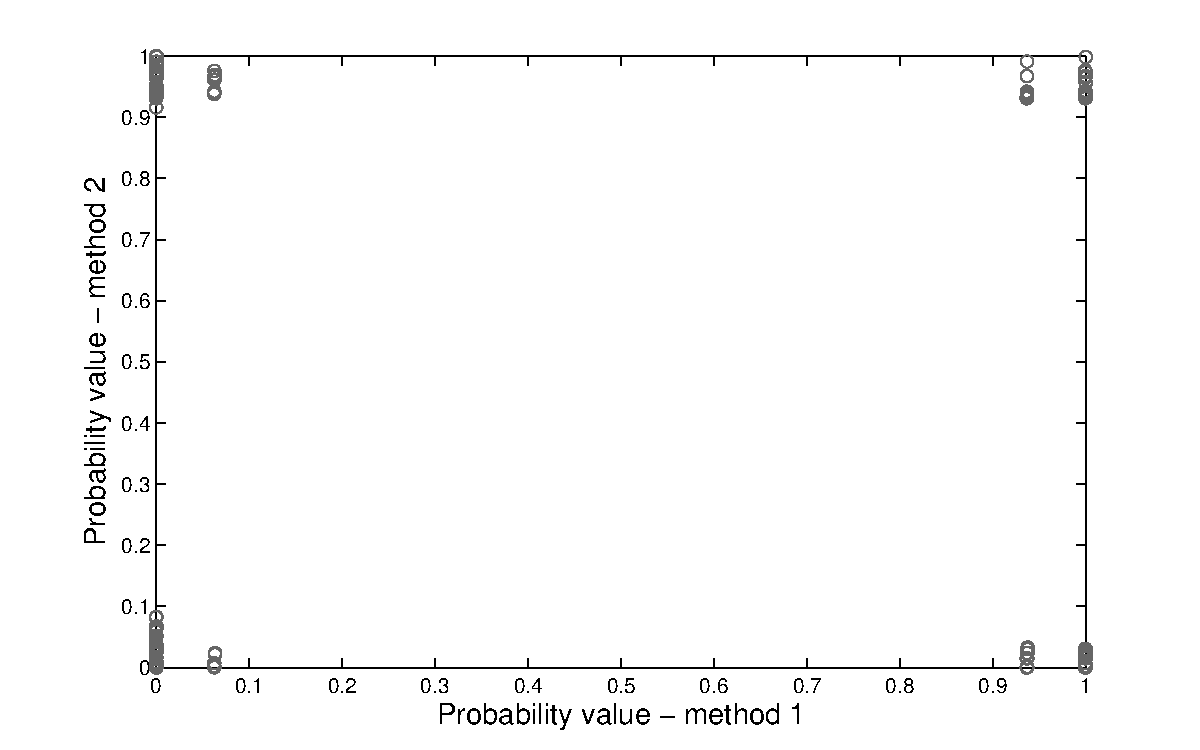
\includegraphics[width=8cm,height=9cm,keepaspectratio]{cloud_Galeras_low.pdf}\\
        (a)
        \end{tabular}
    \end{minipage}
%\hfill
    \begin{minipage}{0.6\textwidth}
        \begin{tabular}{c}
       % \Pic[0.3]{NED30_dem.jpg}\\
	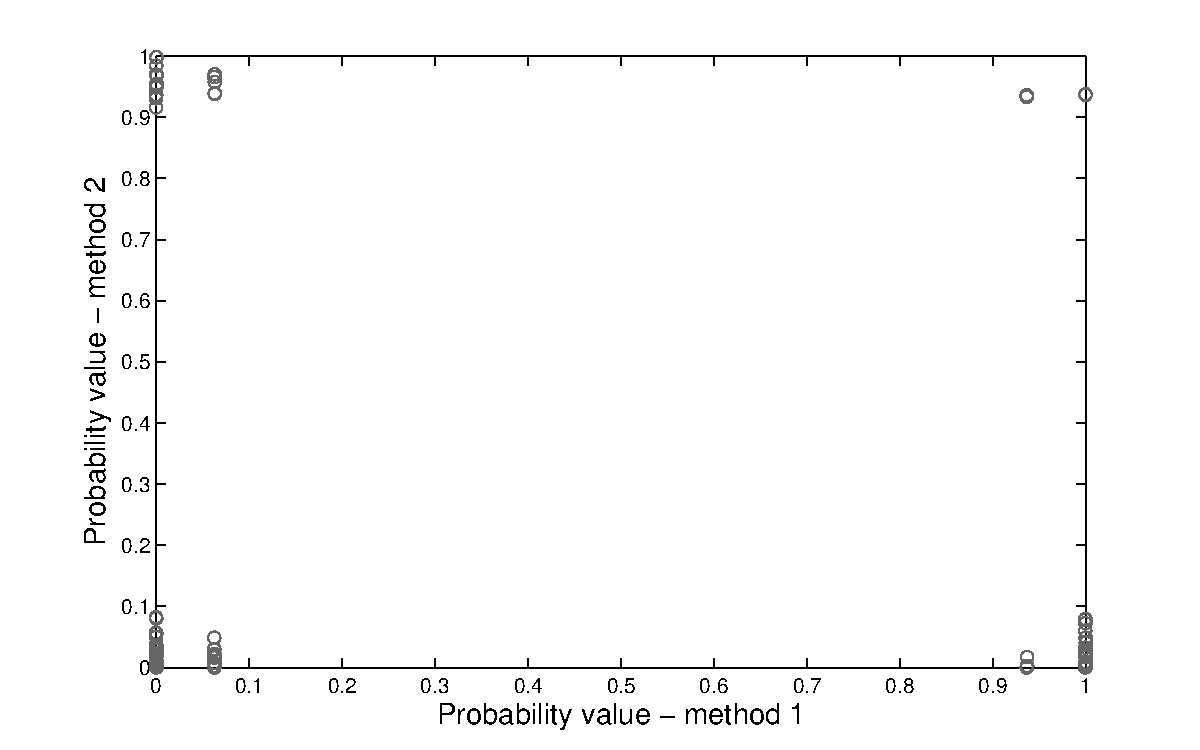
\includegraphics[width=8cm,height=9cm,keepaspectratio]{cloud_Mammoth_low.pdf}\\
        (b)
        \end{tabular}
    \end{minipage} 
        \begin{minipage}[b]{0.6\textwidth}
        \begin{tabular}{c}
       % \Pic[0.3]{SRTM30_dem.jpg}\\
       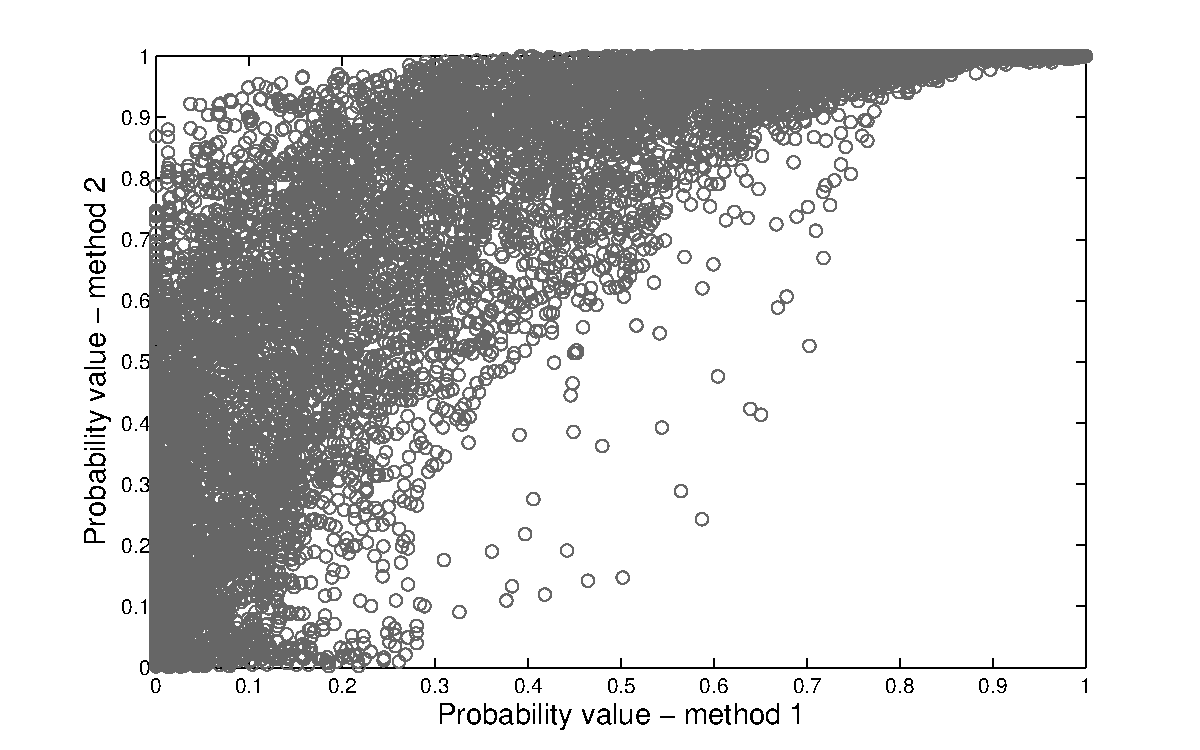
\includegraphics[width=8cm,height=9cm,keepaspectratio]{cloud_Galeras_high.pdf}\\
        (c)
        \end{tabular}
    \end{minipage}
%\hfill
    \begin{minipage}{0.6\textwidth}
        \begin{tabular}{c}
       % \Pic[0.3]{NED30_dem.jpg}\\
	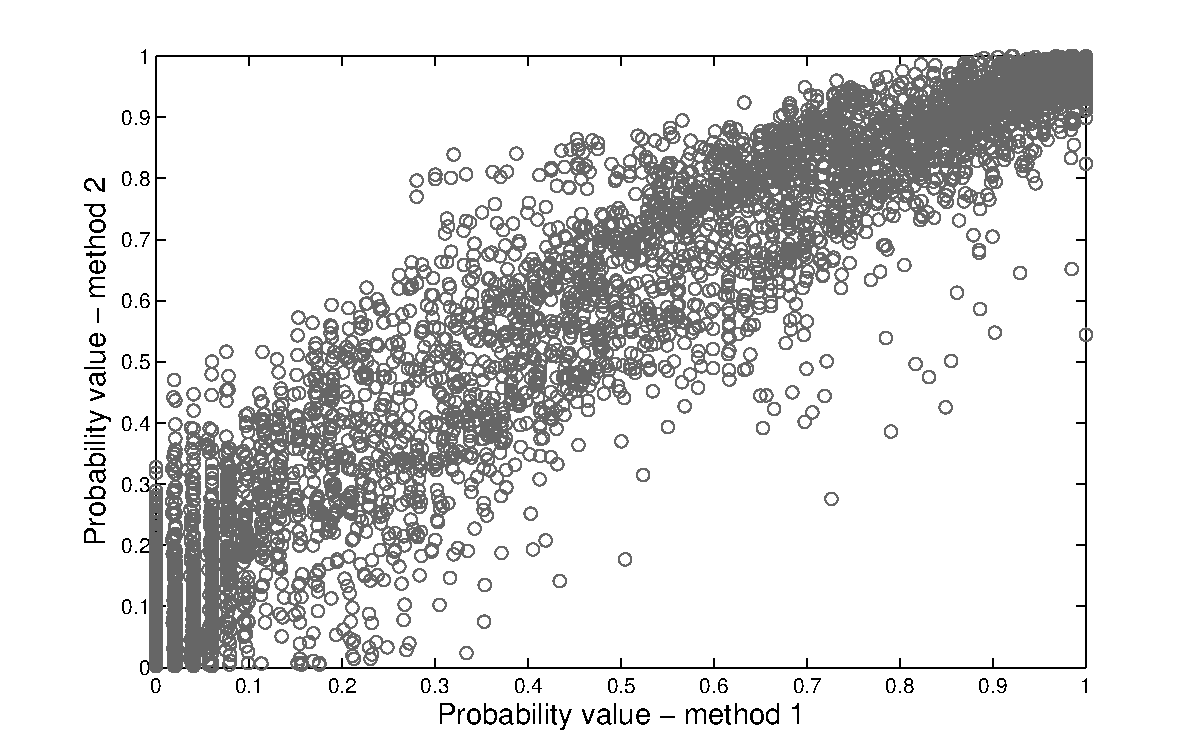
\includegraphics[width=8cm,height=9cm,keepaspectratio]{cloud_Mammoth_high.pdf}\\
        (d)
        \end{tabular}
    \end{minipage}
    \caption{(a) The probability that flow will exceed 0.5 m Method 1
      versus Method 2 for: (a) Galeras Volcano, Colombia for low flow
      (b) Mammoth Mountain, CA for low flow (c) Galeras Volcano,
      Colombia for high flow (d) Mammoth Mountain, CA for high flow }
\label{fig6}  
\end{figure}

%\begin{figure}[H]
%      \begin{minipage}[b]{0.6\textwidth}
%        \begin{tabular}{c}
%       % \Pic[0.3]{SRTM30_dem.jpg}\\
%       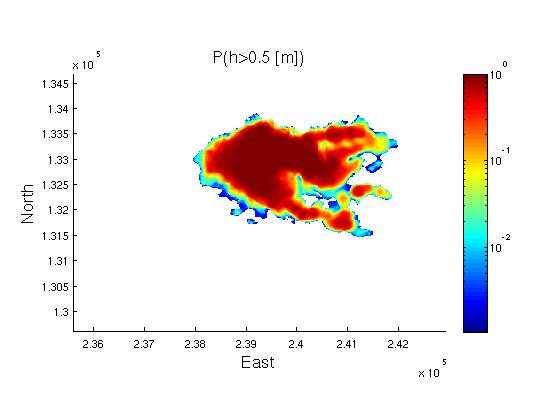
\includegraphics[width=8cm,height=9cm,keepaspectratio]{figs/Galeras_Aster30_P.jpg}\\
%        (a)
%        \end{tabular}
%    \end{minipage}
%%\hfill
%    \begin{minipage}{0.6\textwidth}
%        \begin{tabular}{c}
%       % \Pic[0.3]{NED30_dem.jpg}\\
%	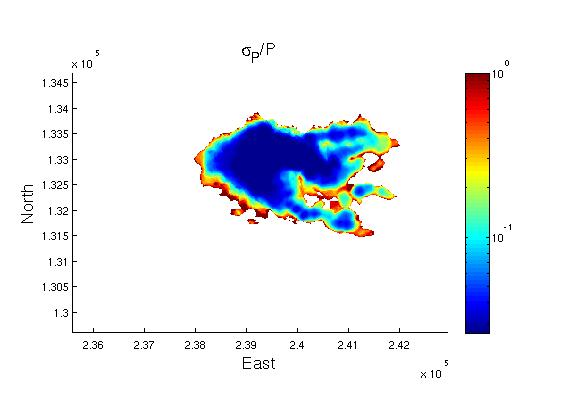
\includegraphics[width=8cm,height=9cm,keepaspectratio]{figs/Galeras_Aster30_sigma.jpg}\\
%        (b)
%        \end{tabular}
%    \end{minipage} 
%     \begin{minipage}[b]{0.6\textwidth}
%        \begin{tabular}{c}
%       % \Pic[0.3]{SRTM30_dem.jpg}\\
%       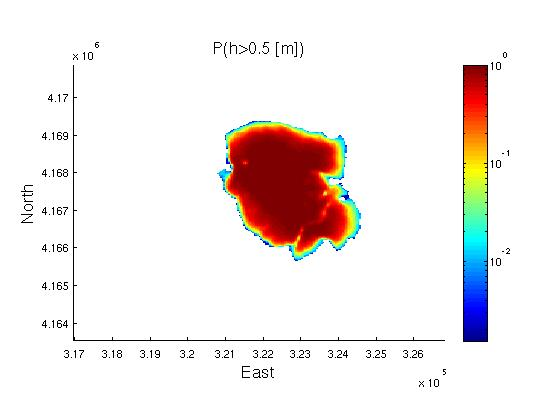
\includegraphics[width=8cm,height=9cm,keepaspectratio]{figs/Mammoth_Topsar30_P.jpg}\\
%        (c)
%        \end{tabular}
%    \end{minipage}
%%\hfill
%    \begin{minipage}{0.6\textwidth}
%        \begin{tabular}{c}
%       % \Pic[0.3]{NED30_dem.jpg}\\
%	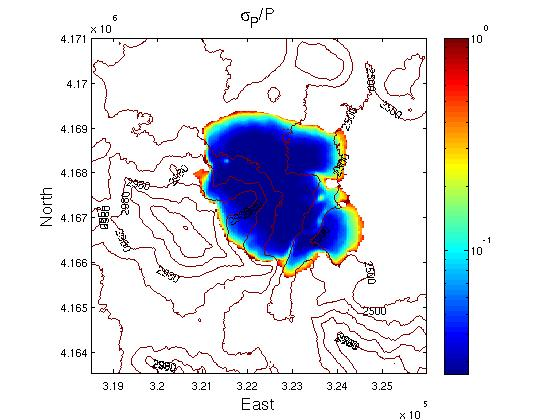
\includegraphics[width=8cm,height=9cm,keepaspectratio]{figs/Mammoth_Topsar30_sigma.jpg}\\
%        (d)
%        \end{tabular}
%    \end{minipage} 
%    \caption{ (a) The probability that flow will exceed 0.5 m for
%      Galeras ASTER (b) Standard deviation in the estimate that the
%      flow will exceed 0.5 m in depth for Galeras ASTER (c) The
%      probability that flow will exceed 0.5 m for Mammoth TOPSAR (d)
%      Standard deviation in the estimate that the flow will exceed 0.5
%      m in depth for Mammoth TOPSAR}
%\label{fig7}  
%\end{figure}

\begin{figure}[H]
      \begin{minipage}[b]{0.6\textwidth}
        \begin{tabular}{c}
       % \Pic[0.3]{SRTM30_dem.jpg}\\
       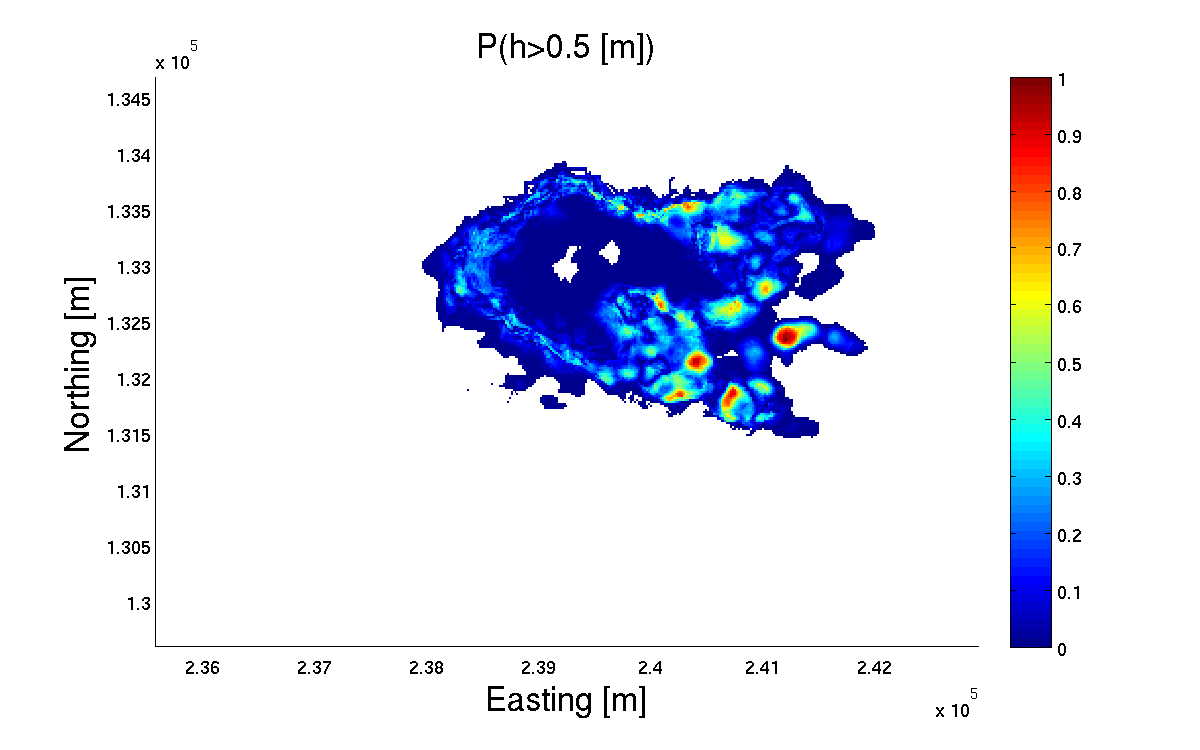
\includegraphics[width=8cm,height=7.5cm,keepaspectratio]{Galeras0_minus_Aster30.pdf}\\
        (a)
        \end{tabular}
    \end{minipage}
%\hfill
    \begin{minipage}{0.6\textwidth}
        \begin{tabular}{c}
       % \Pic[0.3]{NED30_dem.jpg}\\
	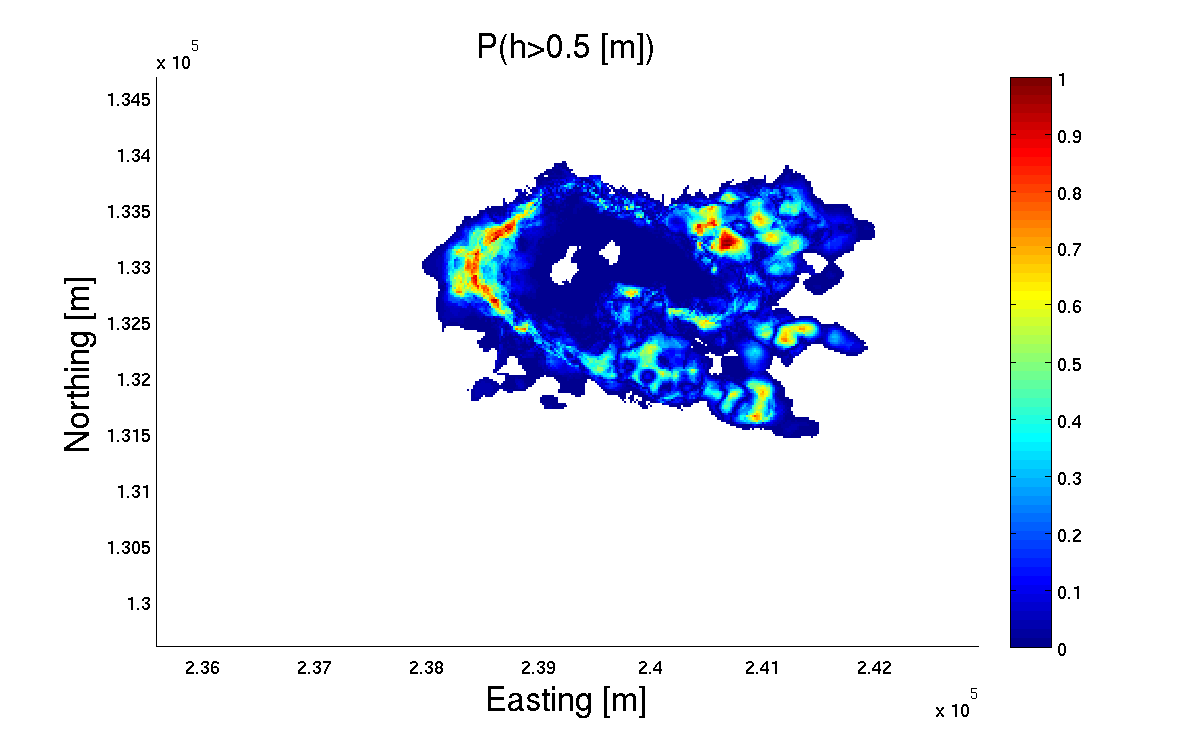
\includegraphics[width=8cm,height=7.5cm,keepaspectratio]{Galeras3_minus_Aster30.pdf}\\
        (b)
        \end{tabular}
    \end{minipage} 
    \begin{minipage}[b]{0.6\textwidth}
        \begin{tabular}{c}
       % \Pic[0.3]{SRTM30_dem.jpg}\\
       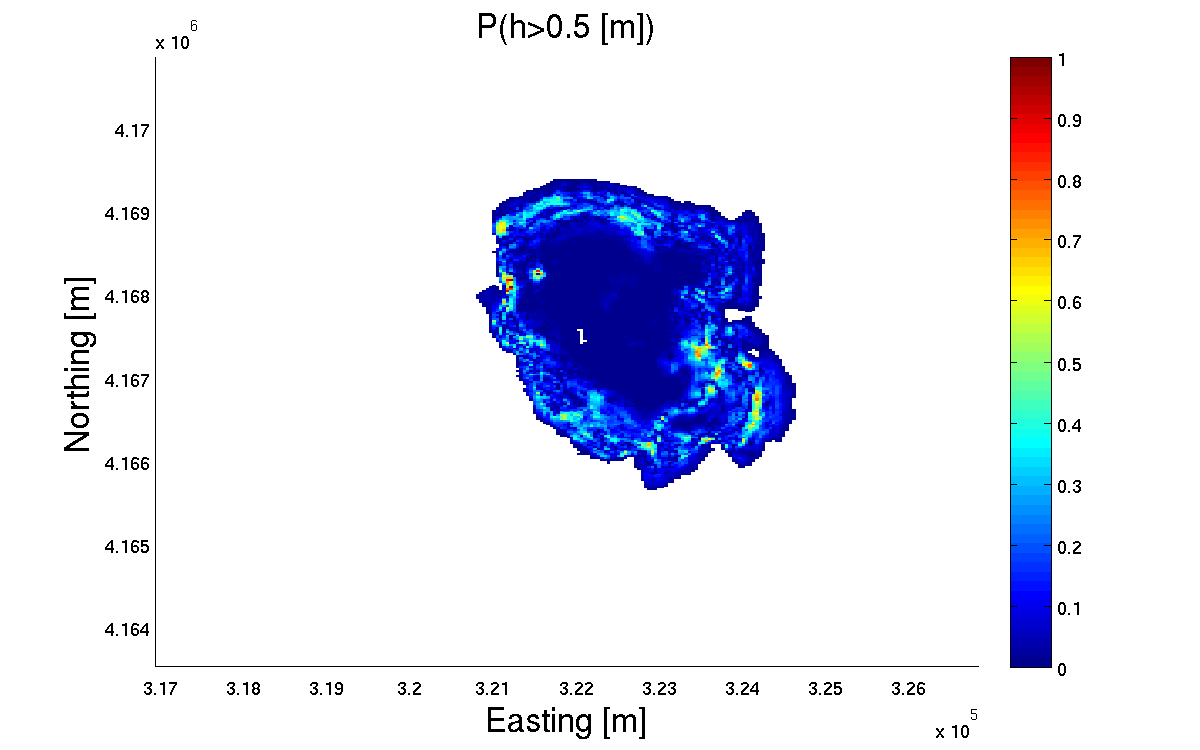
\includegraphics[width=8cm,height=7.5cm,keepaspectratio]{Mammoth0_minus_Aster30.pdf}\\
        (c)
        \end{tabular}
    \end{minipage}
%\hfill
    \begin{minipage}{0.6\textwidth}
        \begin{tabular}{c}
       % \Pic[0.3]{NED30_dem.jpg}\\
	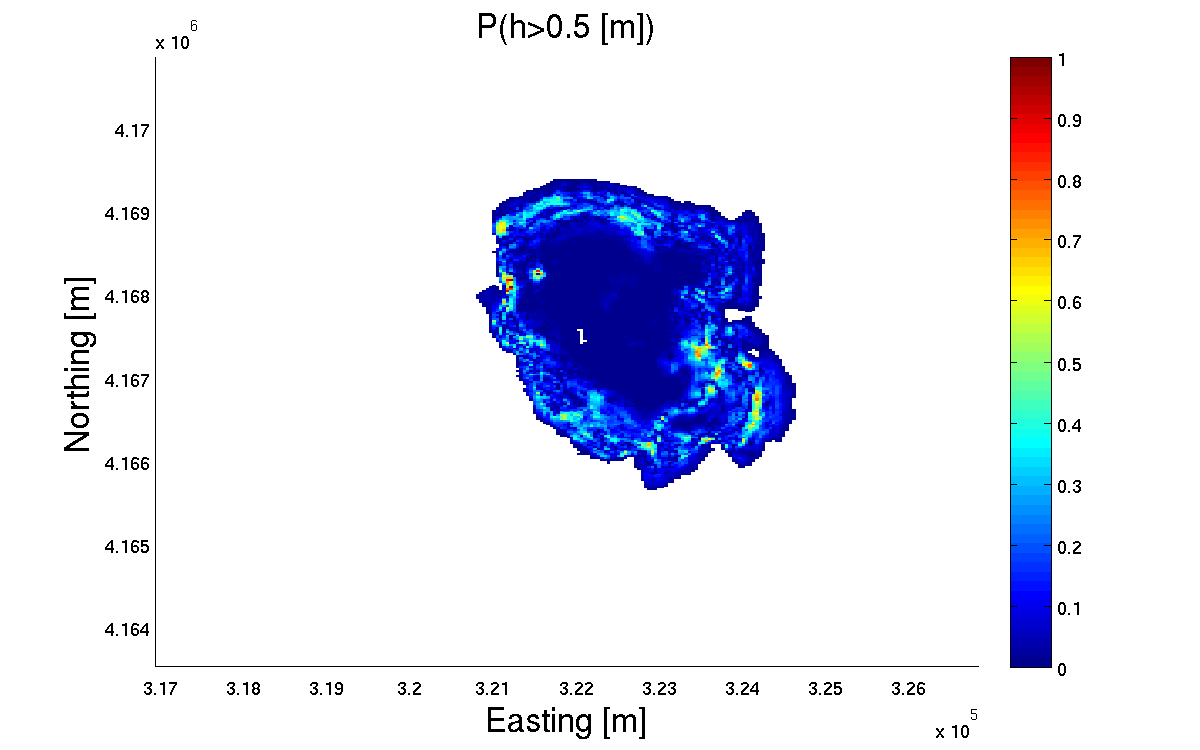
\includegraphics[width=8cm,height=7.5cm,keepaspectratio]{Mammoth0_minus_Aster30.pdf}\\
        (d)
        \end{tabular}
    \end{minipage} 
    \caption{ Probability difference map (absolute value) between: (a)
      Mammoth TOPSAR hazard map and the Method 1 hazard map (b)
      Mammoth TOPSAR hazard map and the Method 2 hazard map (c)
      Galeras ASTER hazard map and the Method 1 hazard map (d) Galeras
      ASTER hazard map and the Method 2 hazard map}
\label{fig8}  
\end{figure}


% see /rainier1/data/ers32/Research_Ramona/second_paper_code/temp_plot/clouds

\begin{figure}[H]
      \begin{minipage}[b]{0.6\textwidth}
        \begin{tabular}{c}
       % \Pic[0.3]{SRTM30_dem.jpg}\\
       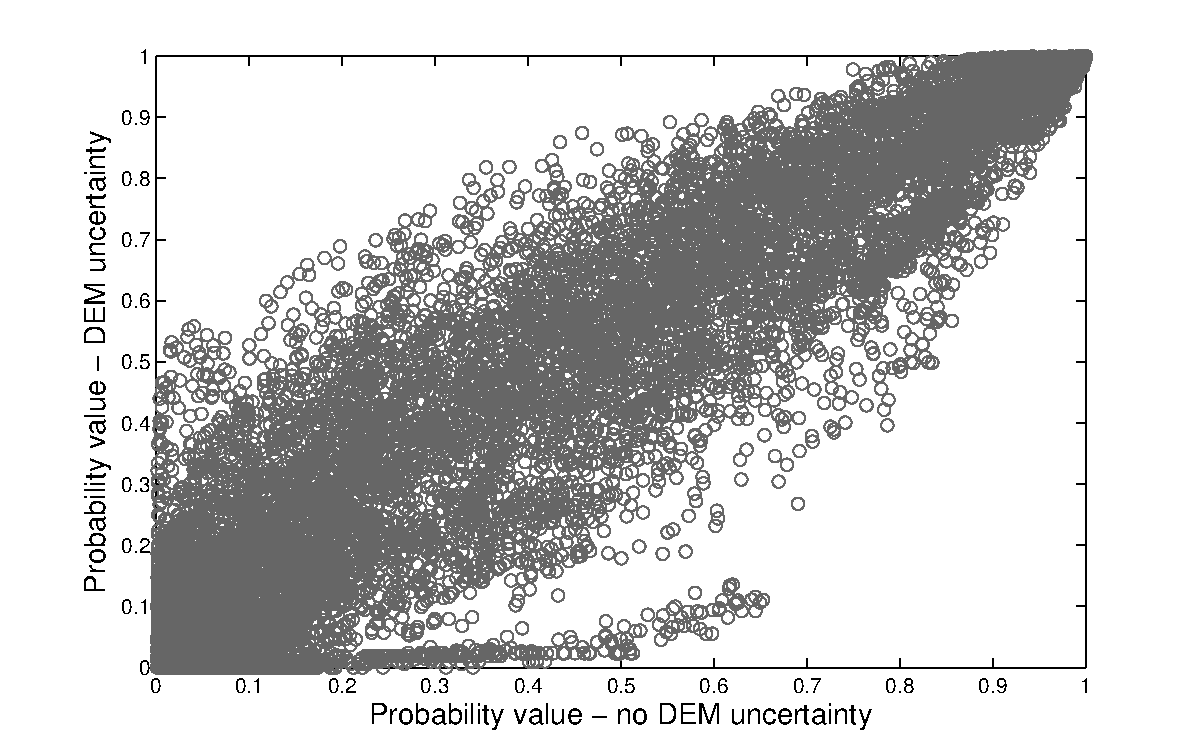
\includegraphics[width=8cm,height=9cm,keepaspectratio]{Galeras_Aster_vs_meth0.pdf}\\
        (a)
        \end{tabular}
    \end{minipage}
%\hfill
    \begin{minipage}{0.6\textwidth}
        \begin{tabular}{c}
       % \Pic[0.3]{NED30_dem.jpg}\\
	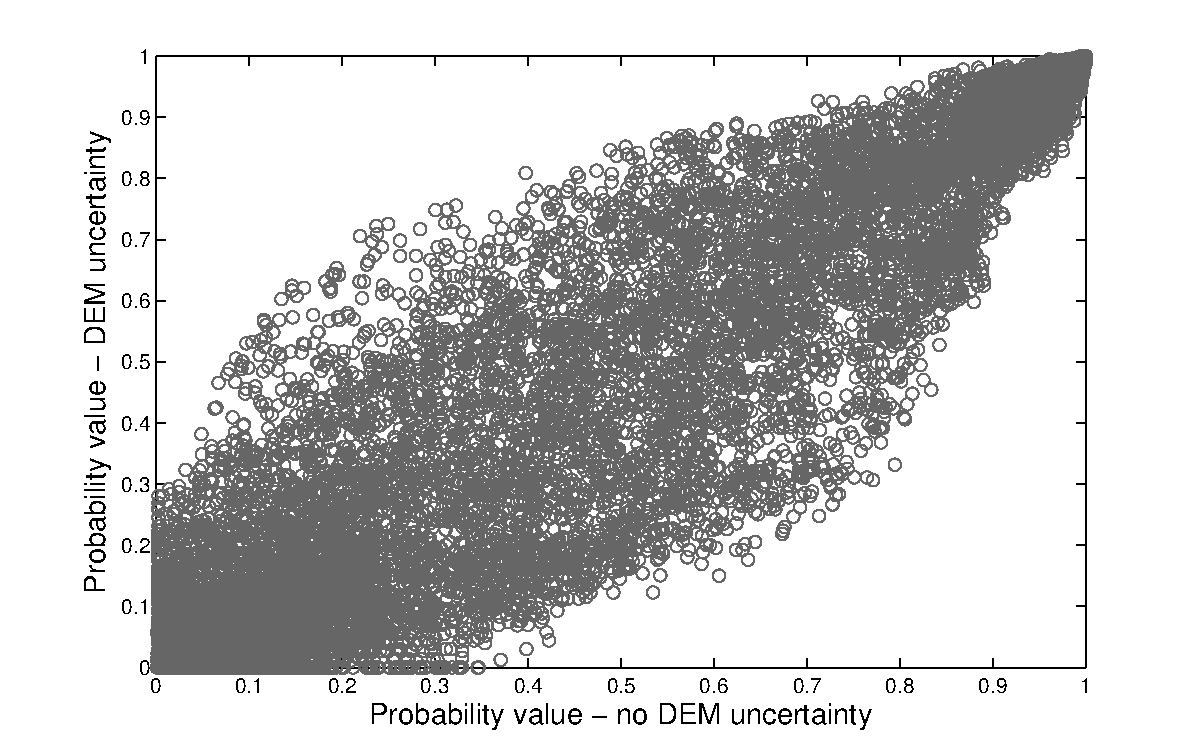
\includegraphics[width=8cm,height=9cm,keepaspectratio]{Galeras_Aster_vs_meth3.pdf}\\
        (b)
        \end{tabular}
    \end{minipage} 
    \begin{minipage}[b]{0.6\textwidth}
        \begin{tabular}{c}
       % \Pic[0.3]{SRTM30_dem.jpg}\\
       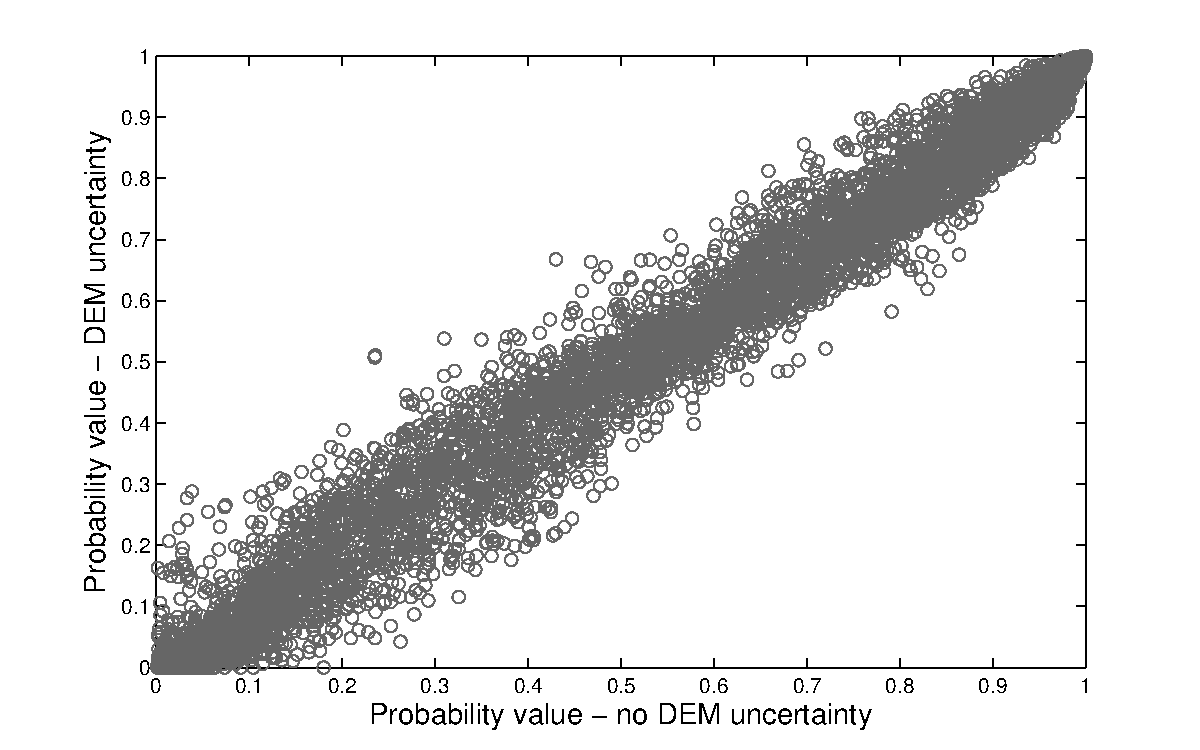
\includegraphics[width=8cm,height=9cm,keepaspectratio]{Mammoth_Topsar_vs_meth0.pdf}\\
        (c)
        \end{tabular}
    \end{minipage}
%\hfill
    \begin{minipage}{0.6\textwidth}
        \begin{tabular}{c}
       % \Pic[0.3]{NED30_dem.jpg}\\
	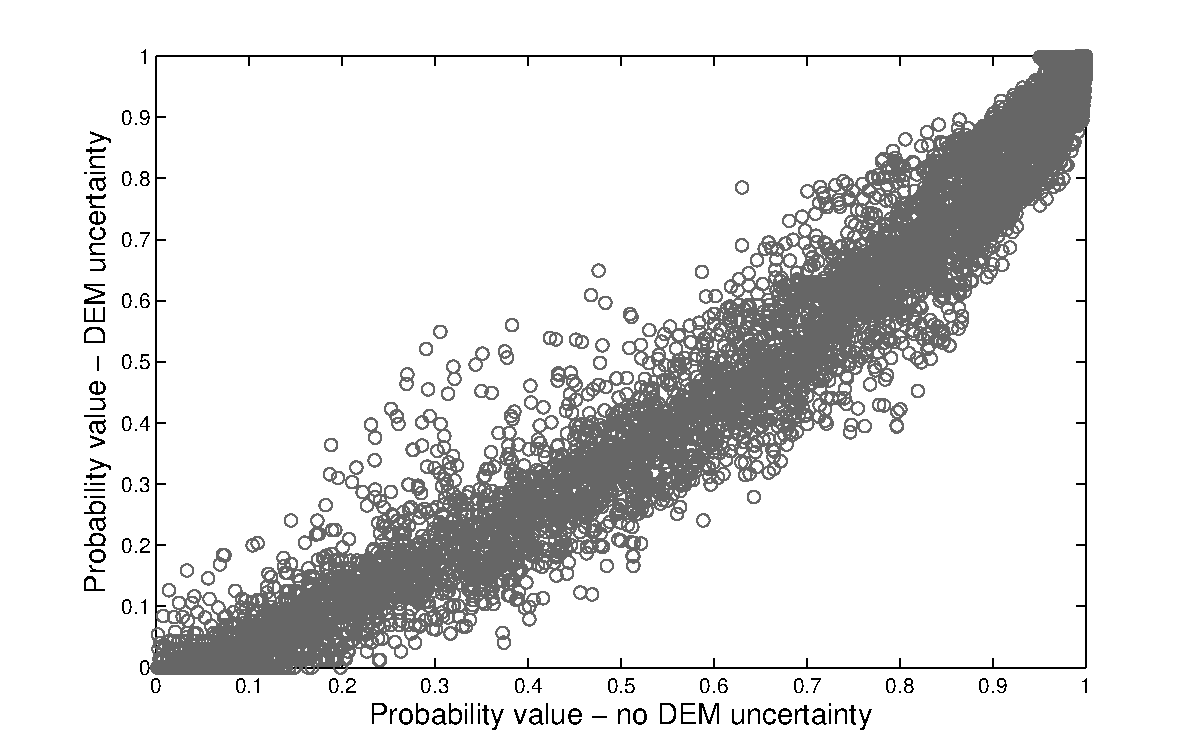
\includegraphics[width=8cm,height=9cm,keepaspectratio]{Mammoth_Topsar_vs_meth3.pdf}\\
        (d)
        \end{tabular}
    \end{minipage} 
    \caption{A comparison of the probability that flow will exceed 0.5
      m when we do not asses for the uncertainty in the DEM and when
      we do, for: (a) Galeras ASTER no DEM uncertainty versus Galeras
      ASTER DEM uncertainty Method 1 (b) Galeras ASTER no DEM
      uncertainty versus Galeras ASTER DEM uncertainty Method 2
      (c) Mammoth TOPSAR - no DEM uncertainty versus Mammoth TOPSAR -
      DEM uncertainty Method 1 (d) Mammoth TOPSAR - no DEM uncertainty
      versus Mammoth TOPSAR - DEM uncertainty Method 2}
\label{fig9}  
\end{figure}

\end{document}
